\documentclass[11pt]{article}

%General
\usepackage{subfiles}
\usepackage{minted}

% Page format
\usepackage[
	top=0.98in,
	bottom=0.98in,
	left=0.98in,
	right=0.98in,
	footskip=26.5pt
]{geometry}
\setlength{\parindent}{0pt}
\linespread{1.5}
\setlength{\parskip}{10.08pt}
\usepackage{pdflscape}

% Math
\usepackage{amsmath}

% Lists and tables
\newcommand{\itemIT}[1]{\item{\textit{#1}\par}}
\newcommand{\itemBF}[1]{\item{\textbf{#1}\par}}
\usepackage{array}
\newcolumntype{L}{>{\bfseries}l}
\newcolumntype{C}{>{\bfseries}c}
\newcolumntype{R}{>{\bfseries}r}
\newcommand{\tabnote}[1]{%
  \multicolumn{2}{p{\dimexpr\linewidth-2\tabcolsep\relax}}{\normalfont #1}\\%
}
\usepackage{enumitem}

% Date
\newcommand{\leadingzero}[1]{\ifnum #1<10 0\the#1\else\the#1\fi}
\newcommand{\todayDMY}{\leadingzero{\day}.\leadingzero{\month}.\the\year}

% Typeface and language
% \usepackage[english]{babel}
\usepackage{helvet}
\renewcommand{\familydefault}{\sfdefault}
\usepackage[T1]{fontenc}
\usepackage{csquotes}
\DeclareQuoteStyle{straight}
  {"}{"}
  {"}{"}
\setquotestyle{straight}

% Colors
\usepackage{xcolor}
\pagecolor{white}
\definecolor{darkblue}{rgb}{0.31,0.53,0.90}
\definecolor{titleBlue}{HTML}{1F355A}
\definecolor{chapterBlue}{HTML}{405E8D}
\definecolor{sectionBlue}{HTML}{5A80B8}

% Sections
\usepackage{titlesec}
\setcounter{secnumdepth}{5}
\titleformat{\section}
{\fontsize{16pt}{19pt}\selectfont\bfseries\color{chapterBlue}}
{\thesection}{1em}{}
\titlespacing*{\section}{0pt}{5pt}{8pt}%
\titleformat{\subsection}
{\fontsize{14pt}{18pt}\selectfont\bfseries\color{chapterBlue}}
{\thesubsection}{0.8em}{}
\titlespacing*{\subsection}{0pt}{5pt}{-5pt}%
\titleformat{\subsubsection}
{\fontsize{11pt}{18pt}\selectfont\bfseries\color{sectionBlue}}
{\thesubsubsection}{0.8em}{}
\titlespacing*{\subsubsection}{0pt}{5pt}{-5pt}%
\titleformat{\paragraph}
{\itshape\fontsize{10.5pt}{14pt}\selectfont\bfseries\color{sectionBlue}}
{\theparagraph}{0.8em}{}
\titlespacing*{\paragraph}{0pt}{6pt}{-5pt}%
\titleformat{\subparagraph}
{\itshape\fontsize{10pt}{10pt}\selectfont\bfseries\color{sectionBlue}}
{\thesubparagraph}{0.5em}{}
\titlespacing*{\subparagraph}{0pt}{0pt}{-10pt}


% TOC
\setcounter{tocdepth}{2}
\usepackage{tocloft}
\renewcommand{\contentsname}{}
\setlength{\cftbeforetoctitleskip}{0pt}
\setlength{\cftaftertoctitleskip}{0pt}
\renewcommand{\cftsecfont}{\normalfont}
\renewcommand{\cftsubsecfont}{\normalfont}
\renewcommand{\cftsubsubsecfont}{\normalfont}
\renewcommand{\cftsecpagefont}{\normalfont}
\renewcommand{\cftsubsecpagefont}{\normalfont}
\renewcommand{\cftsubsubsecpagefont}{\normalfont}
\setlength{\cftbeforesecskip}{2pt}
\setlength{\cftbeforesubsecskip}{1pt}
\setlength{\cftbeforesubsubsecskip}{0pt}
\renewcommand{\cftsecaftersnum}{}
\setlength{\cftparskip}{0pt}
\setlength{\cftbeforetoctitleskip}{0pt}
\setlength{\cftaftertoctitleskip}{10pt}
\renewcommand{\cftaftertoctitle}{}
\renewcommand{\cftdotsep}{0.5}
\renewcommand{\cftsecleader}{\cftdotfill{\cftdotsep}}
\renewcommand{\cftsubsecleader}{\cftdotfill{\cftdotsep}}
\usepackage[hidelinks]{hyperref}
\newcommand{\jtf}[1]{%
    \hyperref[#1]{Jump to reference}%
}

\newcommand{\nocontentsline}[3]{}
\newcommand\stoptoc{%
   \let\origcontentsline\addcontentsline
   \let\addcontentsline\nocontentsline
}
\newcommand\resumetoc{%
   \let\addcontentsline\origcontentsline
}


% References
\usepackage[nameinlink]{cleveref}
\Crefname{subparagraph}{Section}{Sections}
\Crefname{paragraph}{Section}{Sections}
\crefname{figure}{Figure}{Figures}
\newcommand{\fullref}[1]{\textit{\Cref{#1} -- \nameref{#1}}}
\newcommand{\urlCaption}[1]{%
    \vspace{-2mm} \caption*{\small Source: \url{#1}}%
}

% Figures
\usepackage{graphicx}
\usepackage{subcaption}
\graphicspath{{img/}}
\usepackage[skip=2pt]{caption}
\usepackage{subcaption}
\usepackage{multicol}
\usepackage{framed}
\usepackage[export]{adjustbox}

% Appendix
\usepackage{dirtree}

% Bibliography
\usepackage{csquotes}
\usepackage[
	style=numeric,
	backend=biber, 
	sorting=none,
	sortcites=true,
  	maxnames=3,
  	minnames=3
]{biblatex}
\addbibresource{\subfix{bibliography.bib}}
\DefineBibliographyStrings{english}{
  urlseen = {accessed on}
}
\DeclareNameAlias{default}{family-given}

% Cover
\usepackage{titling}
\setlength{\droptitle}{-2.5cm}
\pretitle{%
\begin{center}

\includegraphics[height=.97in]{img/template/ICS_logo.png}

\includegraphics[height=1.94in]{img/template/HdM_logo.png}
\vskip 3em
\linespread{1}\selectfont
\LARGE\bfseries
}
\posttitle{\par\end{center} {\color{sectionBlue}\hrule height 0.6pt} \vspace{-9.5em}}
\title{\textcolor{titleBlue}{\textbf{IT-Sicherheit: Angriff und Verteidigung\\SS2026\\Prof. Dr. Dirk Heuzeroth\\[2em]}}}
\author{}
\date{}

% Footer
\usepackage{etoolbox}
\usepackage{afterpage}
\newif\iflandscapepage
\AtBeginEnvironment{landscape}{%
  \landscapepagetrue
  \thispagestyle{empty}
}
\AtEndEnvironment{landscape}{%
  \afterpage{\landscapepagefalse}
}

\usepackage{fancyhdr}
\pagestyle{fancy}
\fancypagestyle{plain}{
  \fancyhf{}
  \renewcommand{\headrulewidth}{0pt}
  \fancyfoot[R]{\hspace{3cm}\thepage}
  \fancyfootoffset[R]{-2cm}
}
\fancyhf{} \renewcommand{\headrulewidth}{0pt}
\fancyfoot[R]{\hspace{3cm}\thepage}
\fancyfootoffset[R]{-2cm}

\usepackage{tikz}
\AddToHook{shipout/foreground}{%
\begin{tikzpicture}[remember picture,overlay]

\iflandscapepage
  % --- landscape version ---

  % Adjust offsets for 3-digit page numbers
  \ifnum\value{page}>99
    \def\LandscapePageNumberOffset{-1.63cm}
    \def\LandscapeLineOffset{24.85cm}
  \else
    \def\LandscapePageNumberOffset{-1.6cm}
    \def\LandscapeLineOffset{25.05cm}
  \fi

  % page number (upright)
  \node[anchor=south east, rotate=90]
    at ([xshift=\LandscapePageNumberOffset+0.2cm,yshift=25.8cm]current page.south east)
    {\thepage};

  % lines adapted to rotated layout
  {\color{sectionBlue}

  \draw[line width=0.4pt]
    ([yshift=\LandscapeLineOffset]current page.south east)
    -- ([yshift=\LandscapeLineOffset, xshift=51.3em]current page.south west);

  \draw[line width=0.4pt]
    ([yshift=\dimexpr\LandscapeLineOffset+0.05cm\relax]current page.south east)
    -- ([yshift=\dimexpr\LandscapeLineOffset+0.05cm\relax, xshift=51.3em]current page.south west);

  \draw[line width=0.4pt]
    ([yshift=\dimexpr\LandscapeLineOffset+0.10cm\relax]current page.south east)
    -- ([yshift=\dimexpr\LandscapeLineOffset+0.10cm\relax, xshift=51.3em]current page.south west);

  }
  \else
    % --- normal portrait version ---
    \ifnum\value{page}>1
     {\color{sectionBlue}
     
      % Adjust position for 3-digit page numbers
      \ifnum\value{page}>99
       \def\PageLineOffset{-5.25cm}
       \else
       \def\PageLineOffset{-5.05cm}
      \fi
      \draw[line width=0.4pt]
        ([xshift=\PageLineOffset]current page.south east)
        -- ([xshift=\PageLineOffset, yshift=-26.1cm]current page.north east);

      \draw[line width=0.4pt]
        ([xshift=\dimexpr\PageLineOffset-0.05cm\relax]current page.south east)
        -- ([xshift=\dimexpr\PageLineOffset-0.05cm\relax, yshift=-26.1cm]current page.north east);

      \draw[line width=0.4pt]
        ([xshift=\dimexpr\PageLineOffset-0.10cm\relax]current page.south east)
        -- ([xshift=\dimexpr\PageLineOffset-0.10cm\relax, yshift=-26.1cm]current page.north east);
      }
    \fi

  \fi

\end{tikzpicture}%
}

\begin{document}

\maketitle
\thispagestyle{empty}
{\fontsize{16pt}{15pt}\selectfont\color{titleBlue}

\begin{center}
\textbf{Final Report}

Date: \todayDMY
\end{center}

\hfill \break \hfill \break \hfill \break \hfill \break \hfill \break \hfill \break \hfill \break

\begin{tabular}{l l}
\\Name: & \textbf{Neubert, Simon}\\[1em]
Matrikel-Nr. & \textbf{5013322}
\end{tabular}
}

\newpage

\phantomsection
\section*{Ehrenwörtliche Erklärung}
\addcontentsline{toc}{section}{Ehrenwörtliche Erklärung}
Hiermit versichere ich, Simon Neubert, ehrenwörtlich, dass ich den vorliegenden Bericht selbstständig und ohne fremde Hilfe verfasst und keine anderen als die angegebenen Hilfsmittel benutzt habe. Die Stellen des Berichts, die dem Wortlaut oder dem Sinn nach anderen Werken entnommen wurden, sind in jedem Fall unter Angabe der Quelle kenntlich gemacht. Ich versichere, dass ich für die Erstellung dieses Berichts keine KI-Werkzeuge verwendet habe. Der Bericht ist und wird nicht veröffentlicht und er ist bisher auch nicht in dieser oder einer anderen Form als Prüfungsleistung vorgelegt worden.

Ich habe die Bedeutung der ehrenwörtlichen Versicherung und die prüfungsrechtlichen Folgen\\ (§ 24 Abs. 2 Bachelor-SPO) einer unrichtigen oder unvollständigen ehrenwörtlichen Versicherung zur Kenntnis genommen. \\

Stuttgart, den \todayDMY \\[2em]

\includegraphics[height=1.5cm]{template/signature.jpg} \\
Simon Neubert

\newpage

\phantomsection
\section*{Table of Contents}
\addcontentsline{toc}{section}{Table of Contents}
\tableofcontents

\newpage

\section{Executive Summary}
\vspace{-2mm}

\subfile{sections/1.1-bo_summary}

\newpage

\subfile{sections/1.2-pentest_summary}

\newpage

\subfile{sections/1.3-forensics_summary}

\newpage

\subfile{sections/2.1-bo_intro}

\newpage

\subfile{sections/2.2-pentest_intro}

\newpage

\subfile{sections/2.3-forensics_intro}

\newpage

\subfile{sections/3-definitions}

\newpage

\section{Approach / Methodology}

\subfile{sections/4.1-bo_approach}

\newpage

\subfile{sections/4.2-pentest_approach}

\newpage

\subfile{sections/4.3-forensics_approach}

\newpage
 
\section{Vunerabilities and Countermeasures} \label{sec:vuln_counter}
\begin{itemize}
\itemBF{Risk Assessment}
Risk assessment is done via computation of CVSS v4.0 Scores \autocite{first:cvss4}.
The chosen metrics will be explained briefly. 
If a metric isn't listed, it means there is insufficient information to to determine a score and it has been omitted for brevity. \enquote{Not Defined (X)}, \enquote{None (N)}, or \enquote{No (N)} will have be chosen in all such cases.
Environmental Metrics for example are treated as such at points, since they would depend on an actual organization assessing a vulnerability, which doesn't apply to the laboratory setting.
\end{itemize}

\subfile{sections/5.1-bo_vulns}

\newpage

\subsection{Linux - Complete Pentest (Mesa)}

\newpage

\subsection{Digital Forensics}

\newpage

\section{Personal Evaluation}

\subfile{sections/6.1-bo_eval}

\subfile{sections/6.2-pentest_eval}

\subfile{sections/6.3-forensics_eval}

\newpage

\section{References}

\printbibliography[heading=none]

\newpage
\section{Appendix} \label{Appendix}
\stoptoc

\subsection{Buffer Overflow}  \label{Appendix-1}
The appendix provided as a directory is laid out the following way, containing the following content:
\\
\dirtree{%
.1 Final Report - Simon Neubert/.
.2 Windows Scanning and Buffer Overflow.
.3 Nmap Scan.
.4 nmap.txt.
.4 nmap-3389.txt.
.3 vulnserver\_script.
.4 unique\_charseq.txt.
.4 vulnserver-poc-orig.py.
}

\normalsize
\begin{itemize}
\item{The subdirectory \enquote{Nmap scan} the output generated by Nmap (nmap.txt and nmap-3389.txt).}
\item{The subdirectory \enquote{vulnserver\_script} contains the python script used to execute the attack, and the resources it accessed during runtime.}\\
It was altered during the assignment, and all relevant steps have been left in the code and labeled with comments.
\end{itemize}

\newpage
\begin{landscape}
\begin{figure}[h]
\makebox[1.01\linewidth][c]{%
	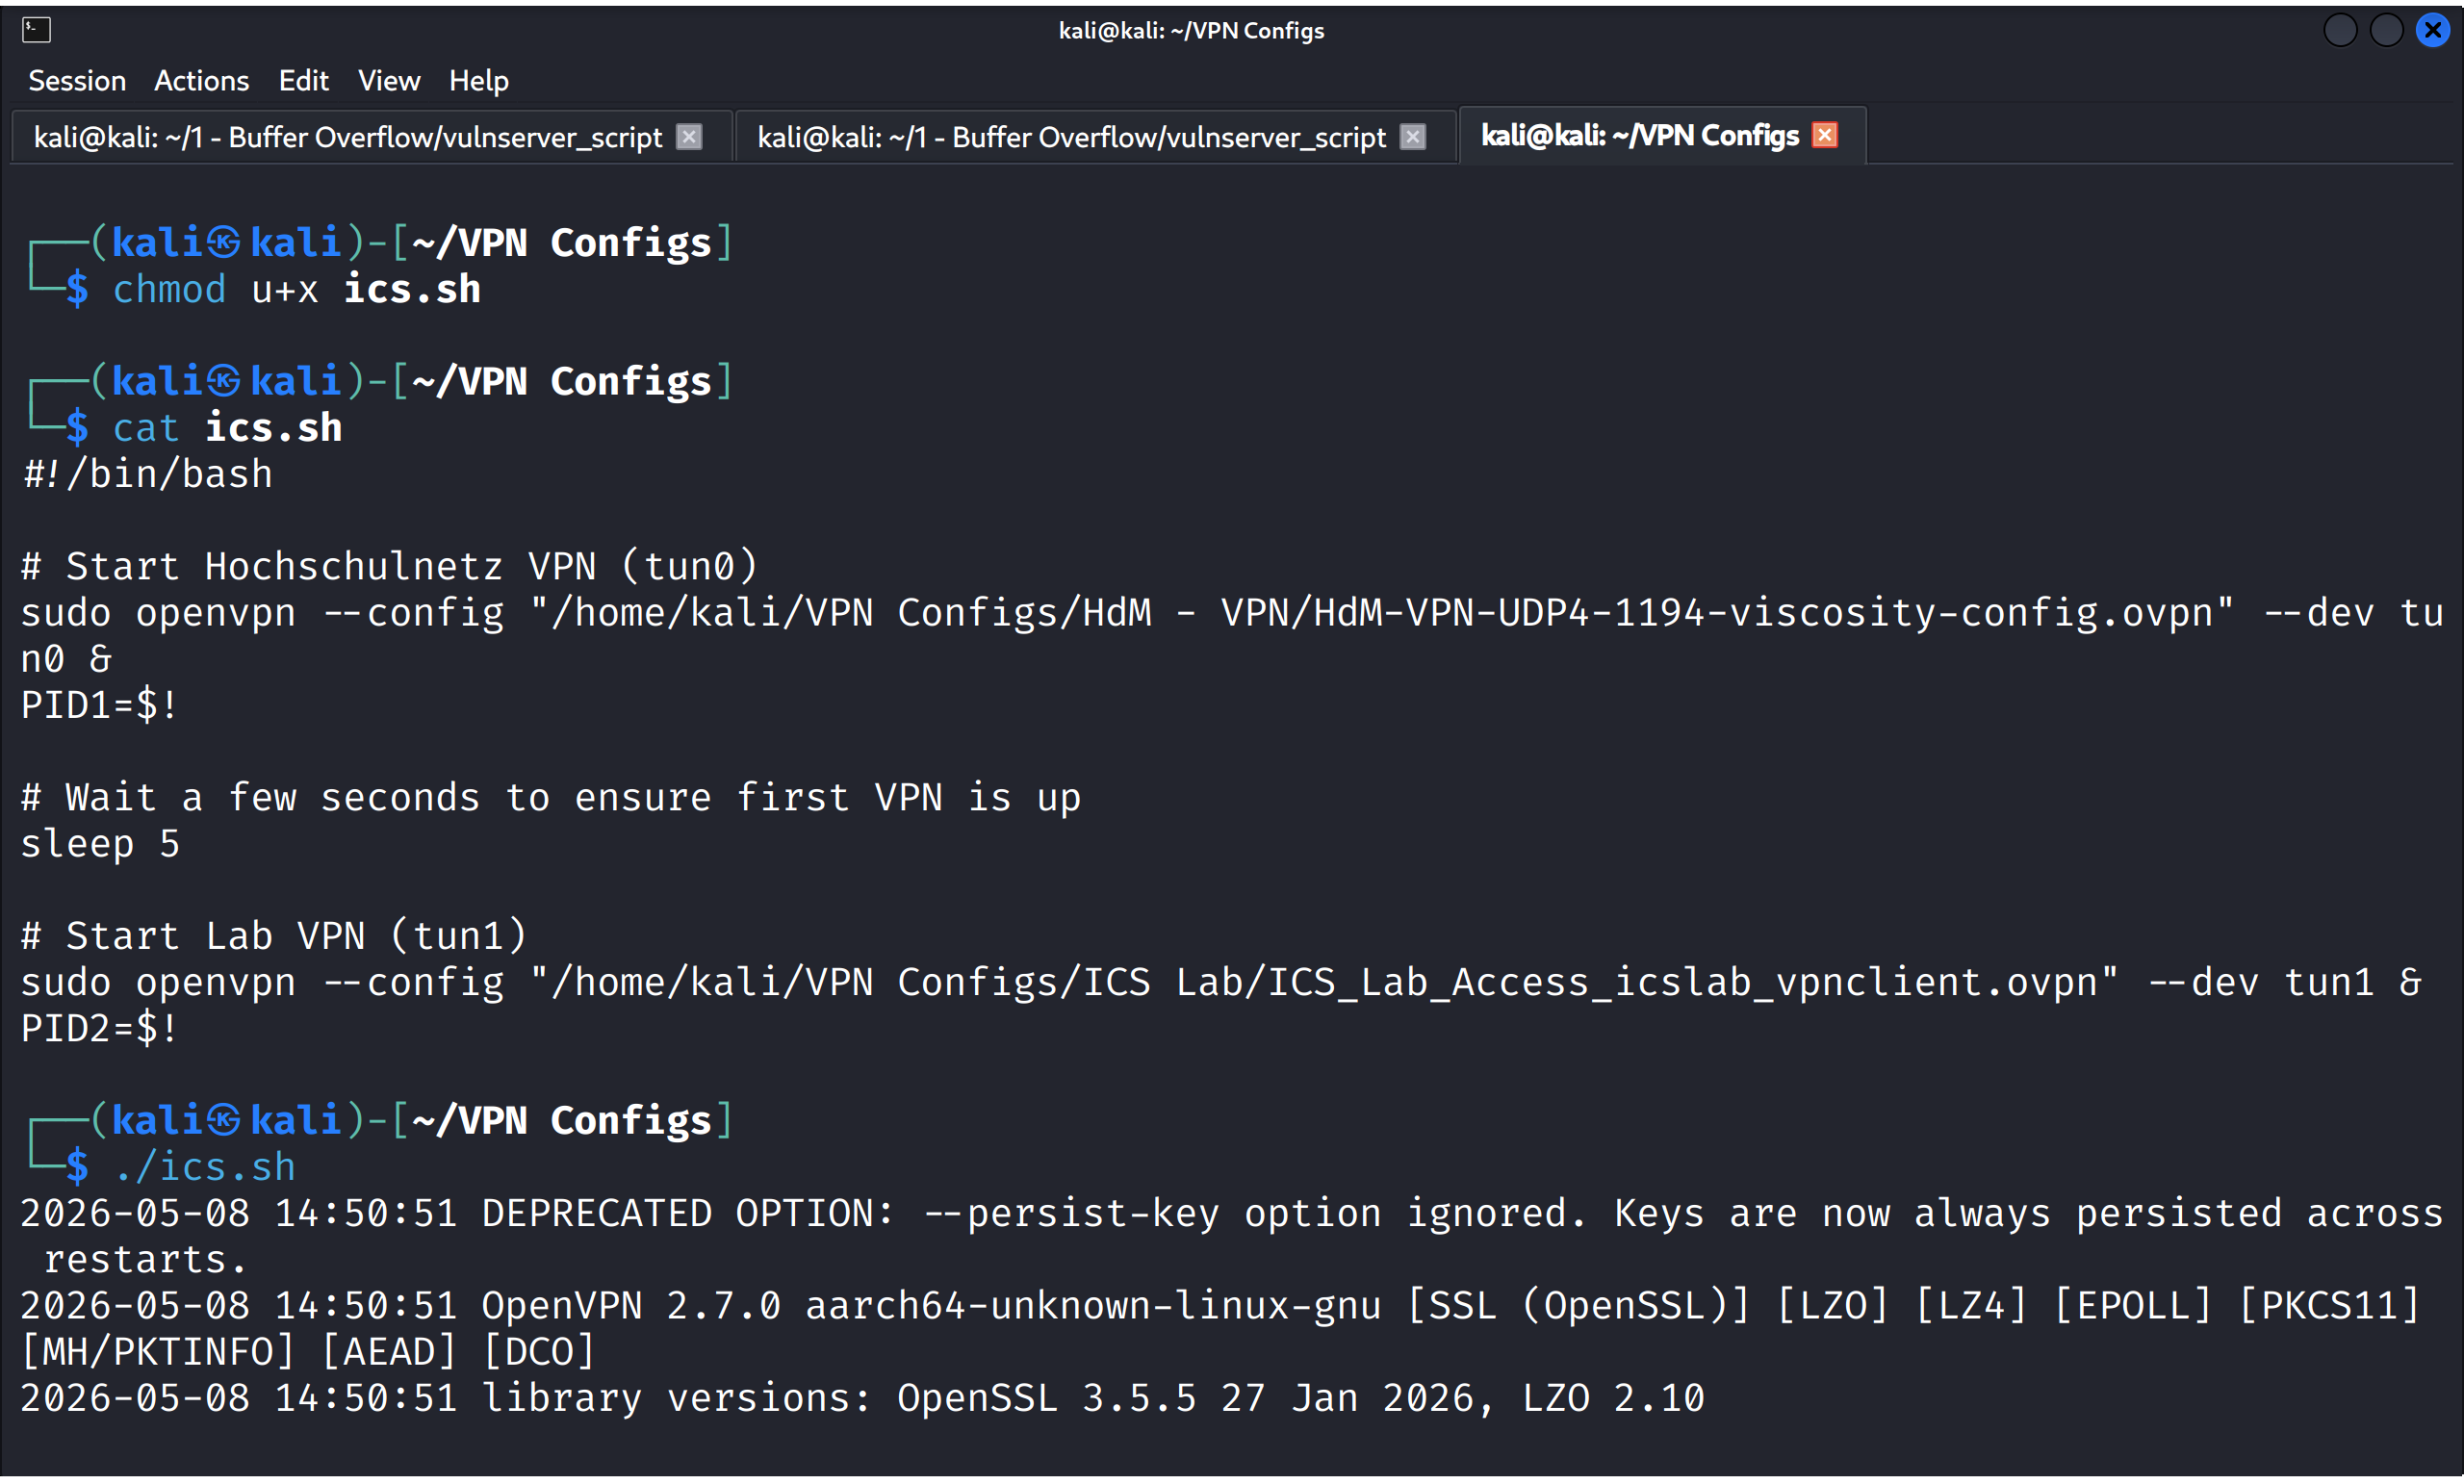
\includegraphics[width=1.15\linewidth]{buffer_overflow/flimsy/0_vpn1}
}
\caption{VPN configuration on an attacker machine not provided by the HdM}
\label{private_vpn1}
\end{figure}

\begin{figure}[h]
\makebox[1.01\linewidth][c]{%
	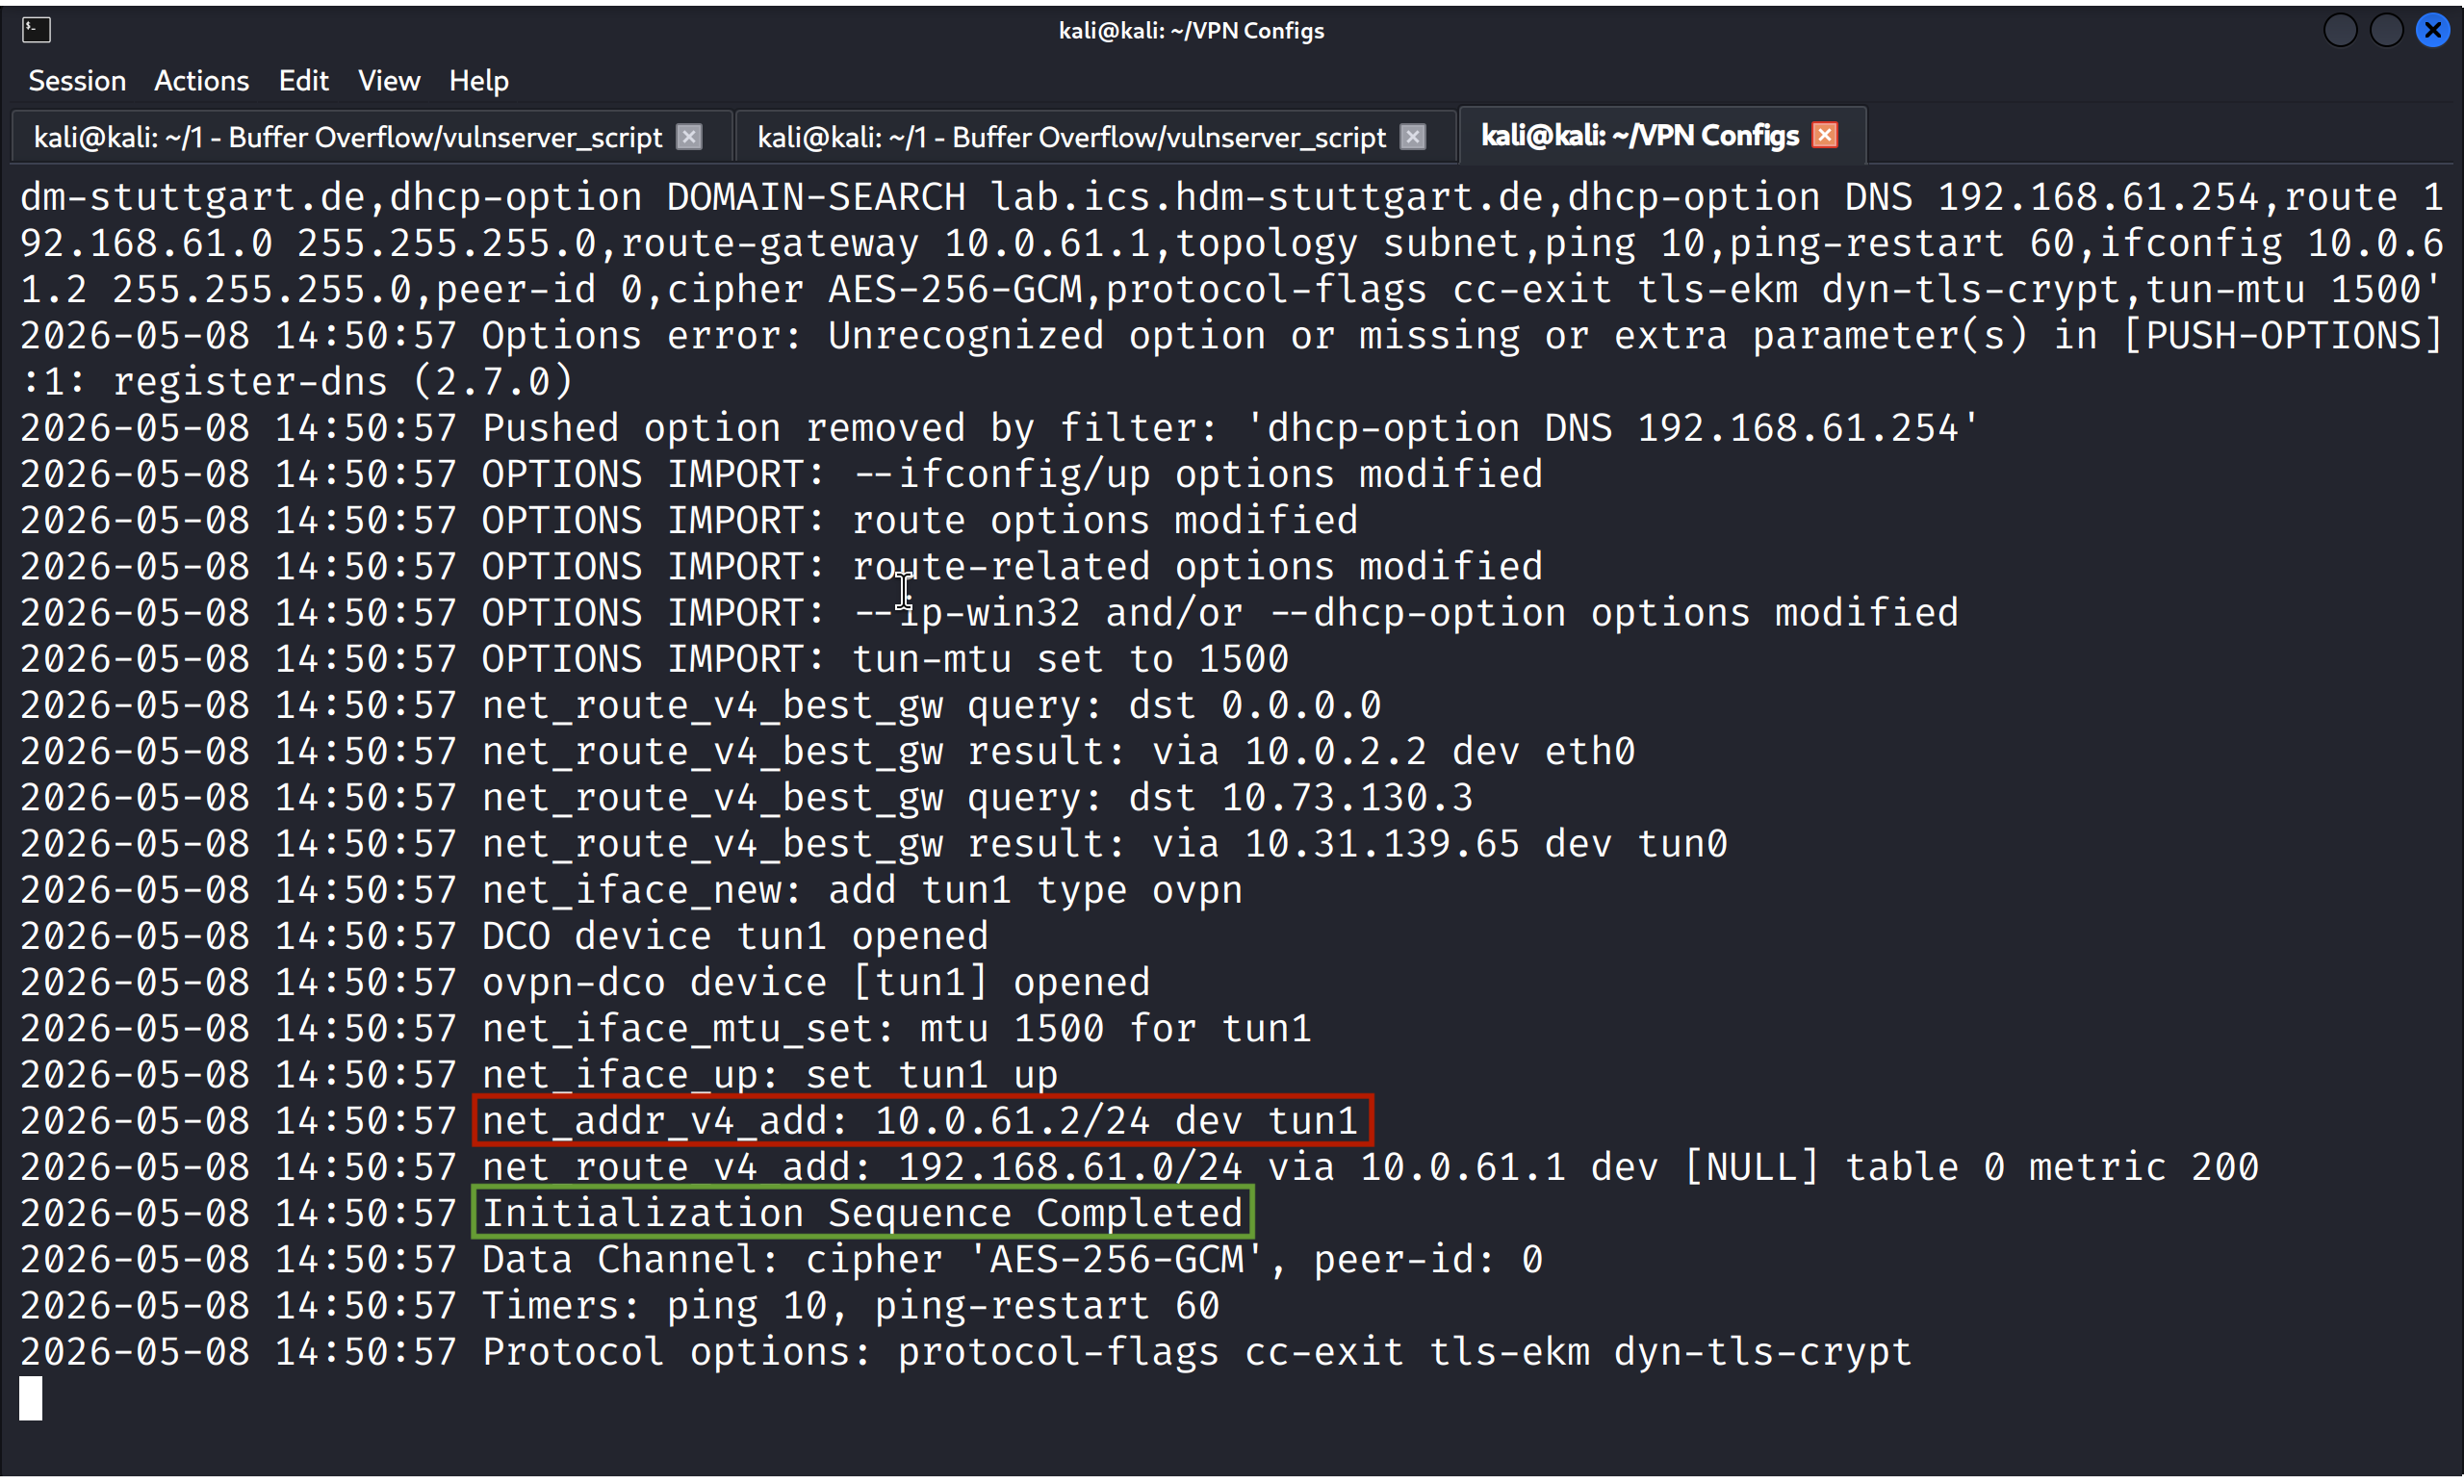
\includegraphics[width=1.15\linewidth]{buffer_overflow/flimsy/0_vpn2}
}
\caption{VPN connected on attacker machine not provided by the HdM with IP 10.0.61.2}
\end{figure}
\end{landscape}

\begin{figure}[h]
\makebox[1.01\linewidth][c]{%
	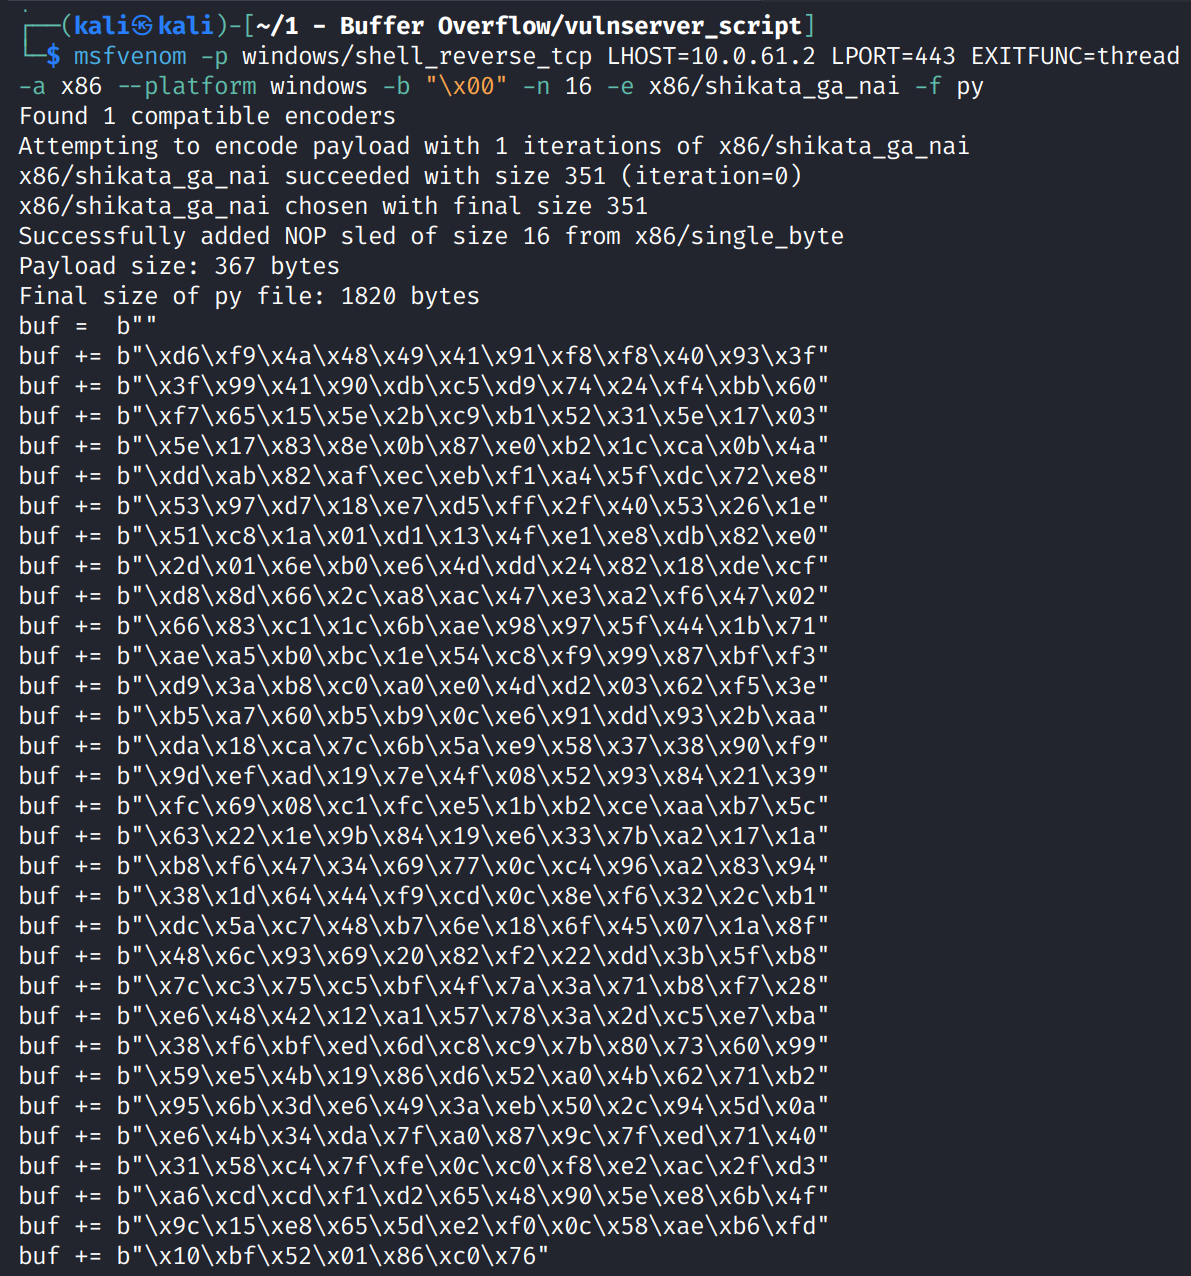
\includegraphics[width=1.15\linewidth]{buffer_overflow/flimsy/1_generate}
}
\caption{Payload generation on attacker machine}
\end{figure}

\begin{figure}[h]
\makebox[1.01\linewidth][c]{%
	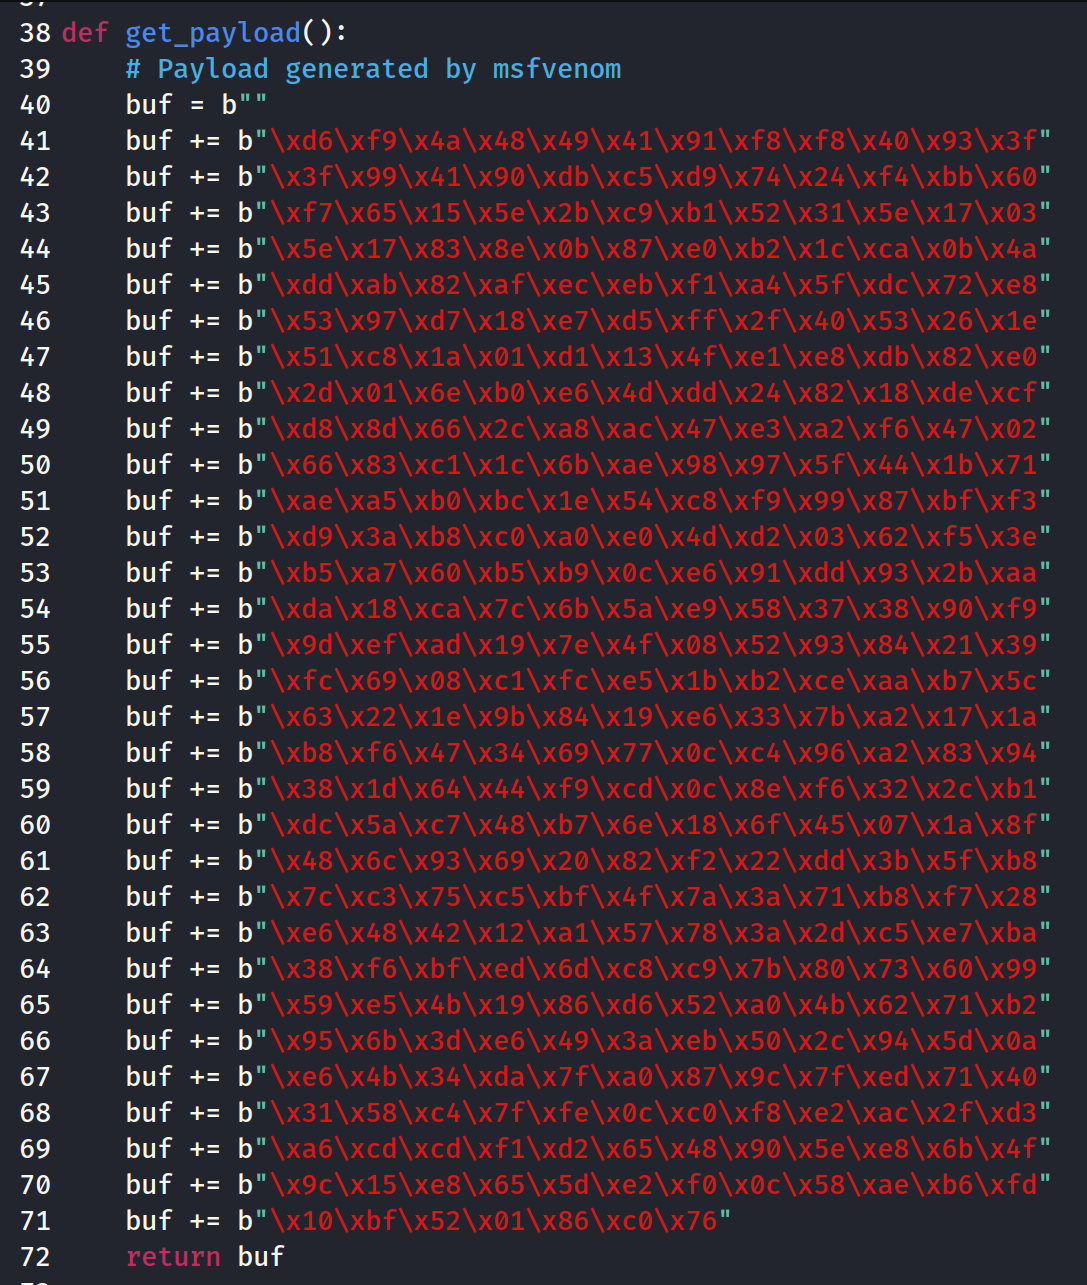
\includegraphics[width=1.15\linewidth]{buffer_overflow/flimsy/1_payload}
}
\caption{Payload used in python script on attacker machine}
\end{figure}

\newpage

\begin{landscape}
\begin{figure}[!h]
\makebox[1.01\linewidth][c]{%
	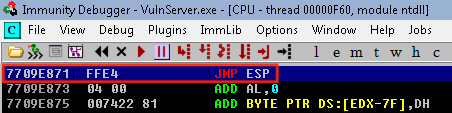
\includegraphics[width=1.15\linewidth]{buffer_overflow/flimsy/2_pre_jmp}
}
\caption{Impermanent JMP ESP instruction located at 7709E871, pre-restart}
\end{figure}

\begin{figure}[!h]
\makebox[\linewidth][c]{%
	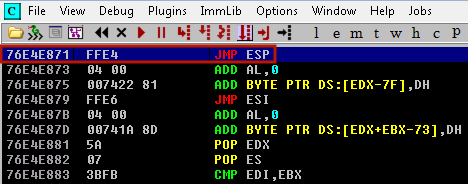
\includegraphics[width=1.15\linewidth]{buffer_overflow/flimsy/2_jmp_esp}
}
\caption{Impermanent JMP ESP instruction located at 76E4E871, post-restart}
\end{figure}

\begin{figure}[!h]
\makebox[\linewidth][c]{%
	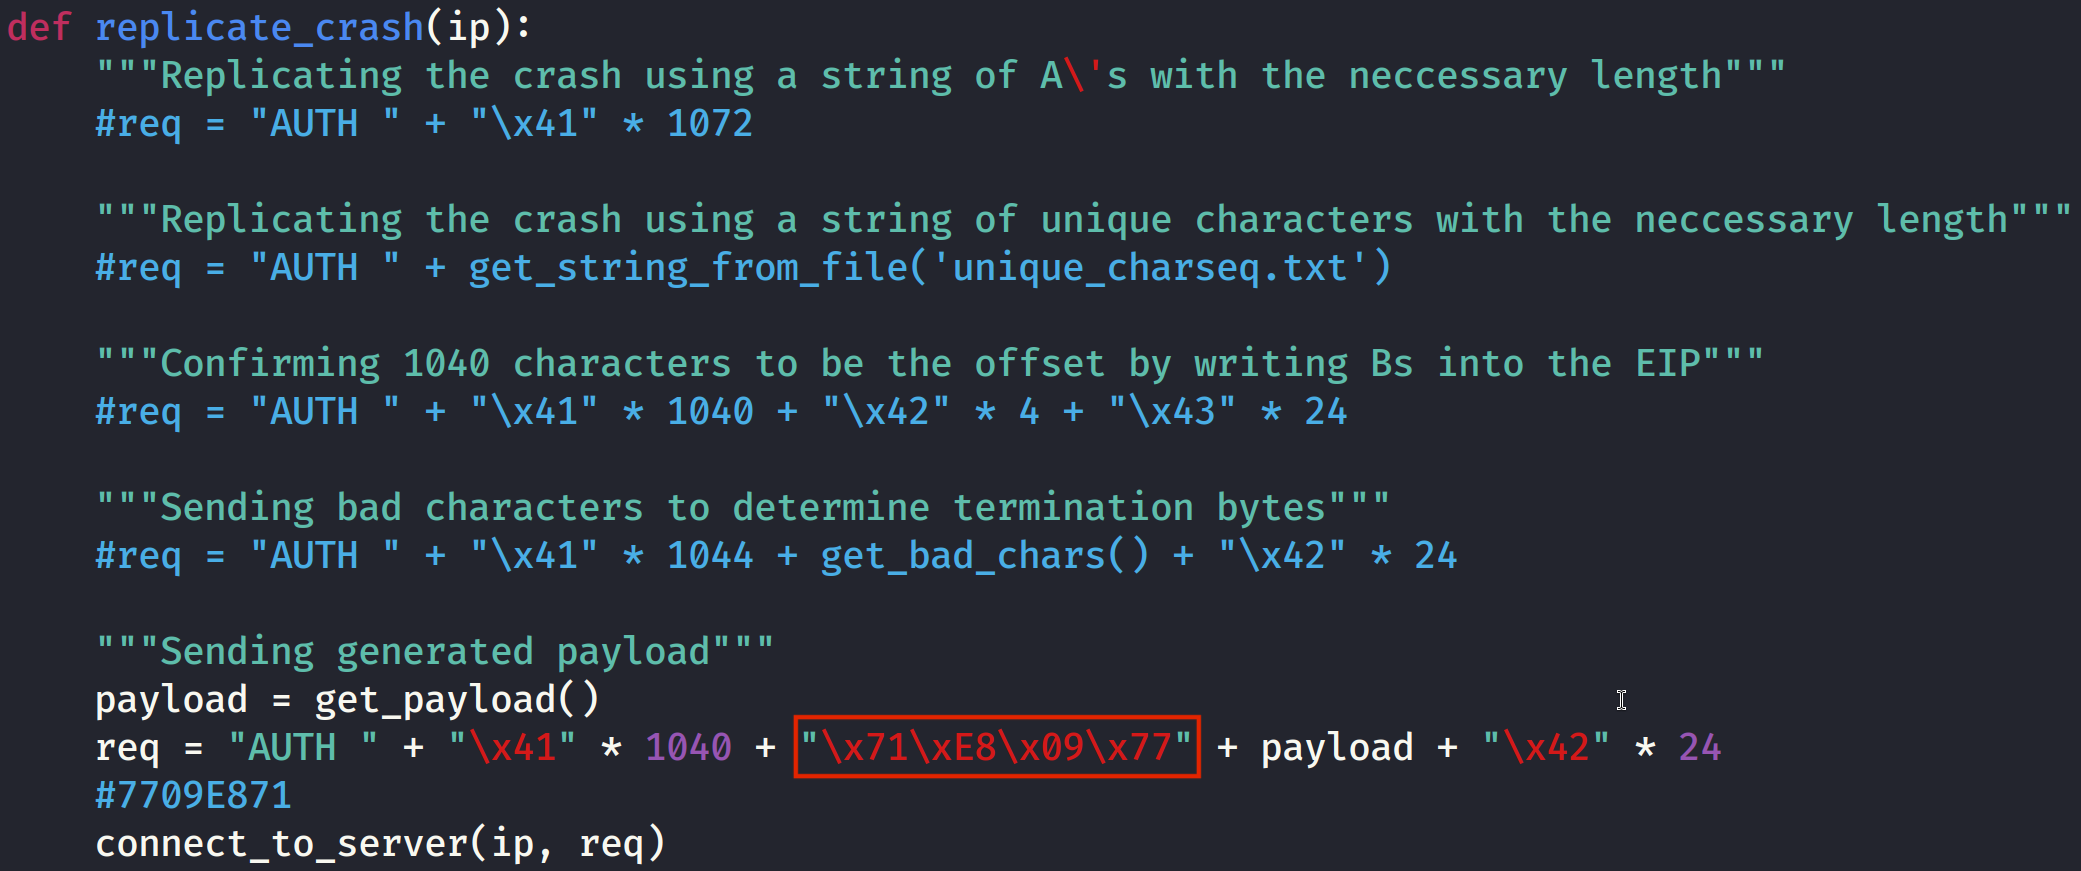
\includegraphics[width=1.15\linewidth]{buffer_overflow/flimsy/pre_address/0_script}
}
\caption{Using impermanent JMP ESP instruction location found before the restart in attack script}
\label{fail_start}
\end{figure}

\begin{figure}[!h]
\makebox[1.01\linewidth][c]{%
	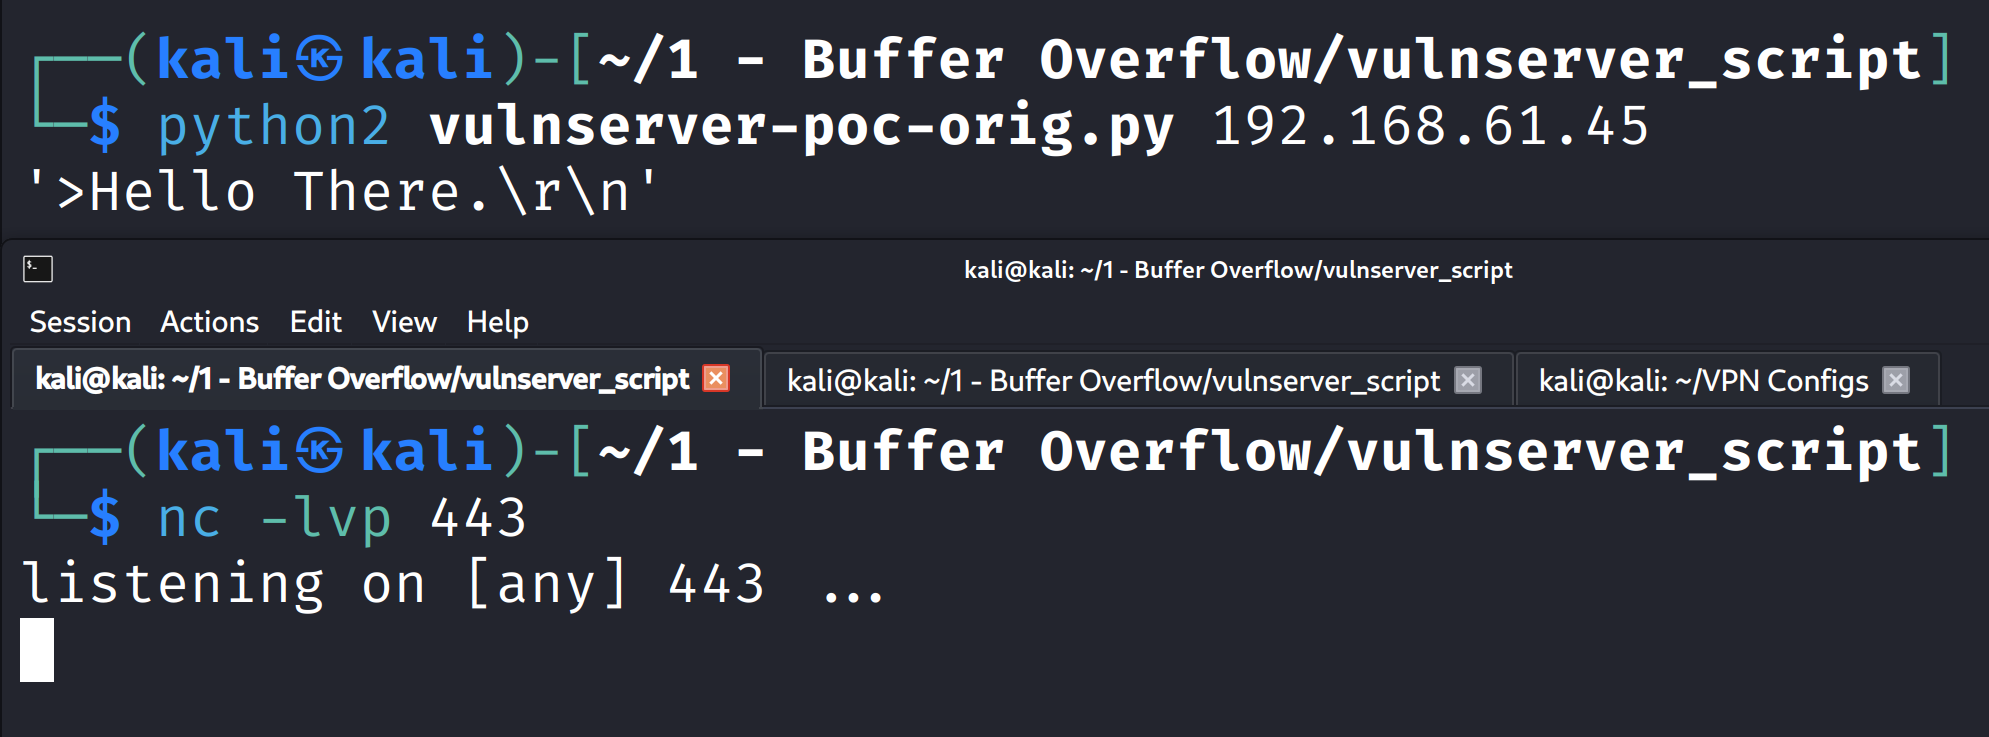
\includegraphics[width=1.15\linewidth]{buffer_overflow/flimsy/pre_address/2_no_conn}
}
\caption{No reverse shell when attacking with the old JMP ESP address post restart}
\label{fail_end}
\end{figure}

\begin{figure}[!h]
\makebox[1.01\linewidth][c]{%
	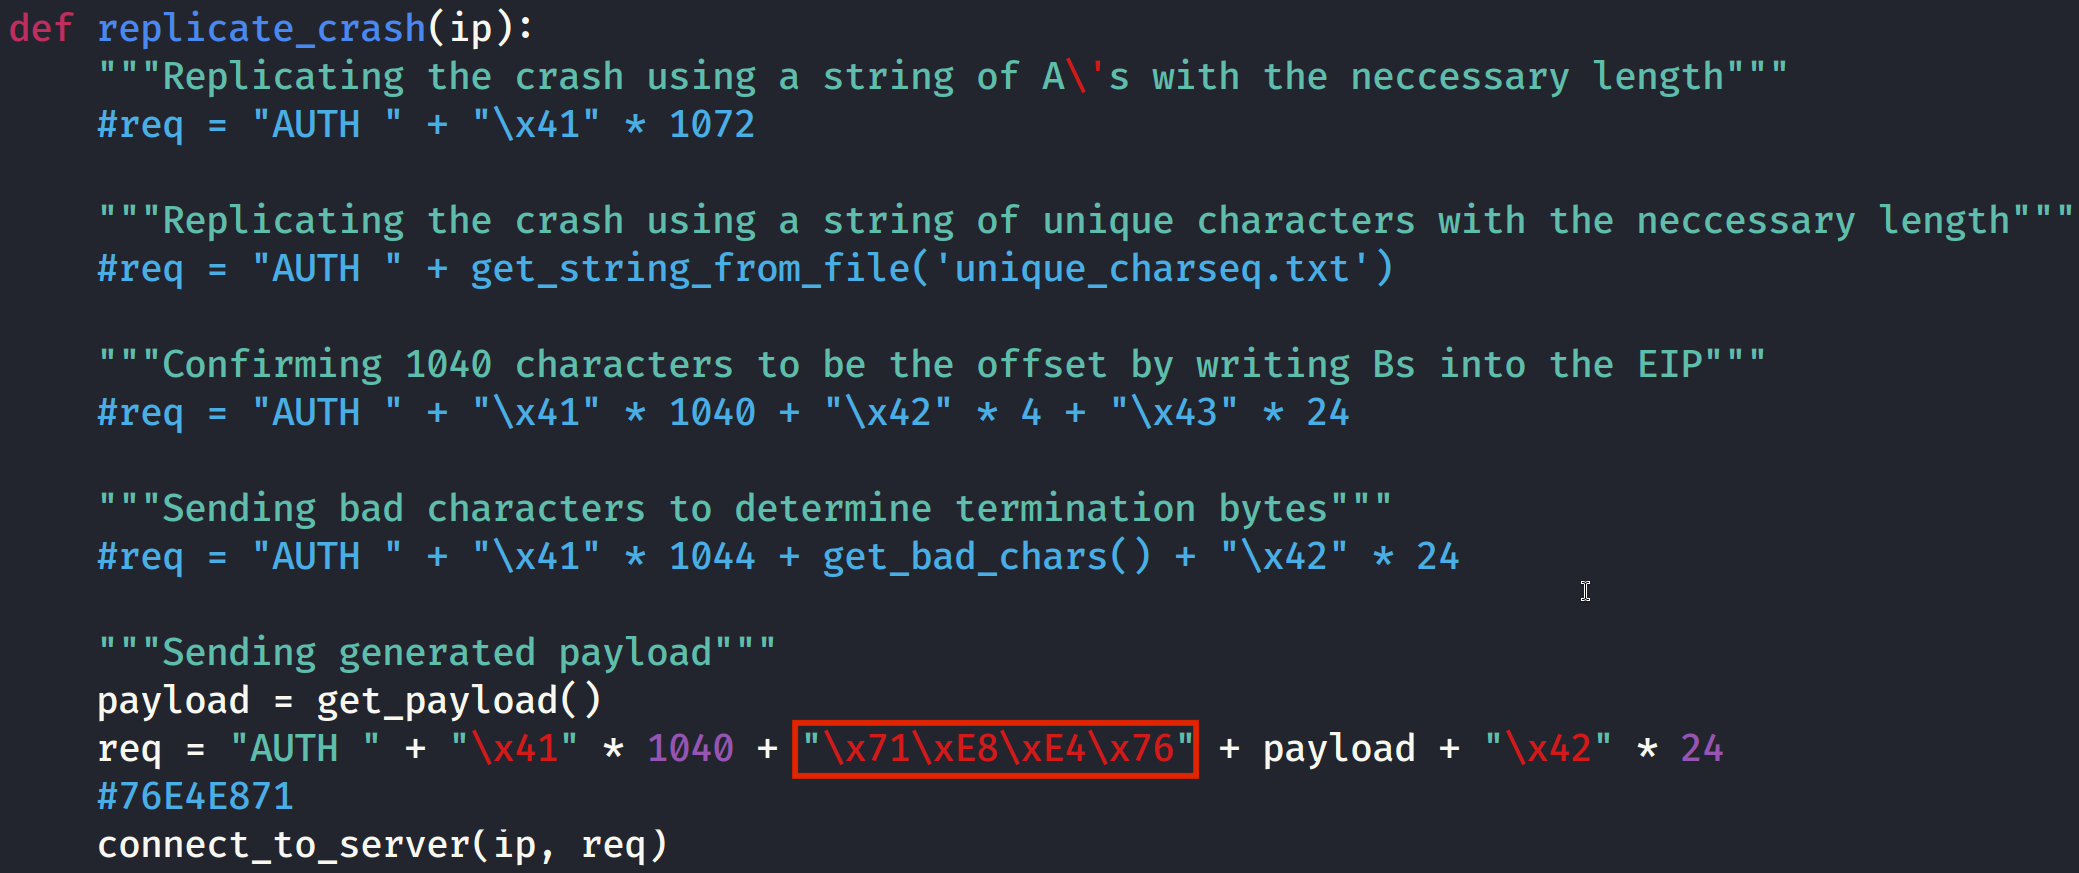
\includegraphics[width=1.15\linewidth]{buffer_overflow/flimsy/3_code}
}
\caption{Using impermanent JMP ESP instruction location found after the restart in attack script}
\end{figure}

\begin{figure}[!h]
\makebox[1.01\linewidth][c]{%
	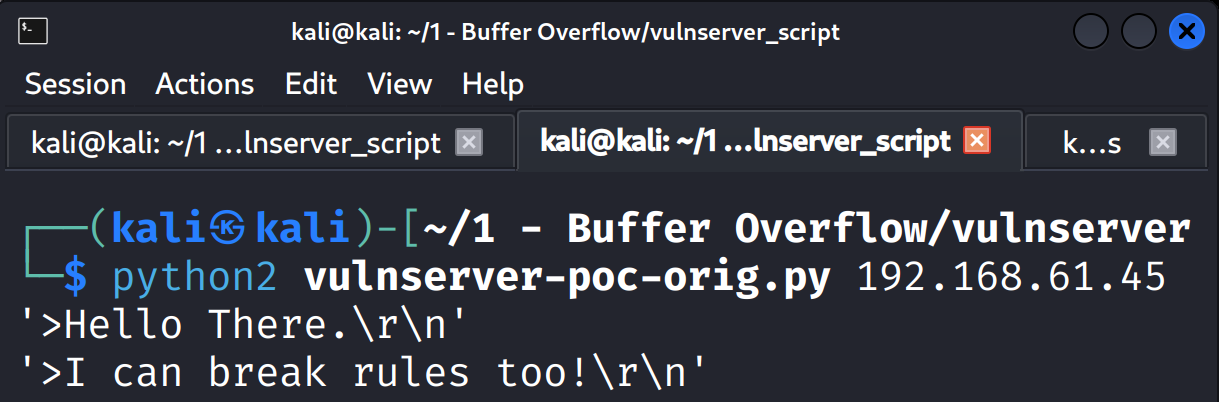
\includegraphics[width=1.15\linewidth]{buffer_overflow/flimsy/3_run}
}
\caption{Running attack using the impermanent address found after the restart}
\end{figure}

\begin{figure}[!h]
\makebox[1.01\linewidth][c]{%
	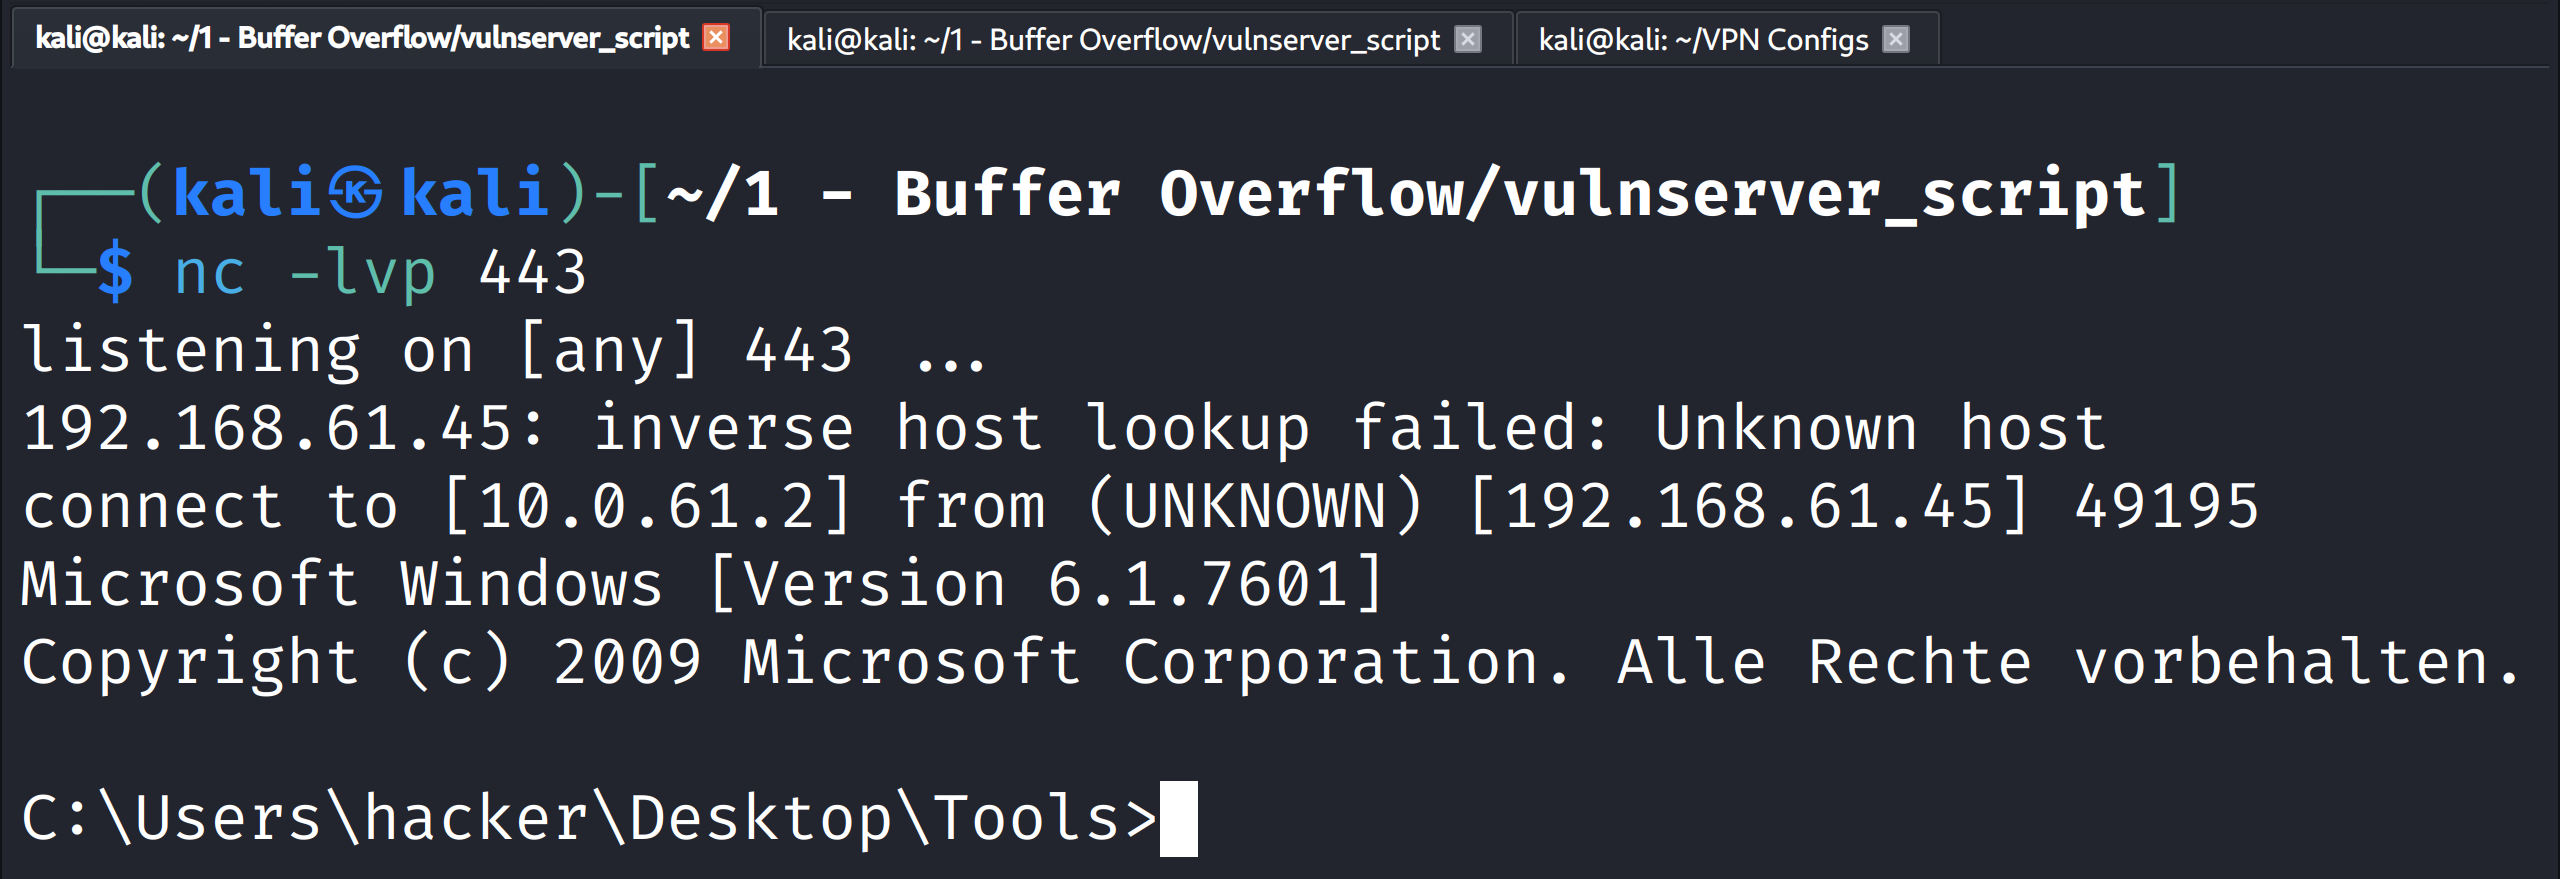
\includegraphics[width=1.15\linewidth]{buffer_overflow/flimsy/4_shell}
}
\caption{Reverse shell created by exploiting the impermanent post-restart JMP ESP location}
\label{reverse_foreign}
\end{figure}
\end{landscape}

\subsection{Linux - Complete Pentest (Mesa)}  \label{Appendix-2}

\begin{figure}[!htb]
\makebox[1.01\linewidth][c]{%
	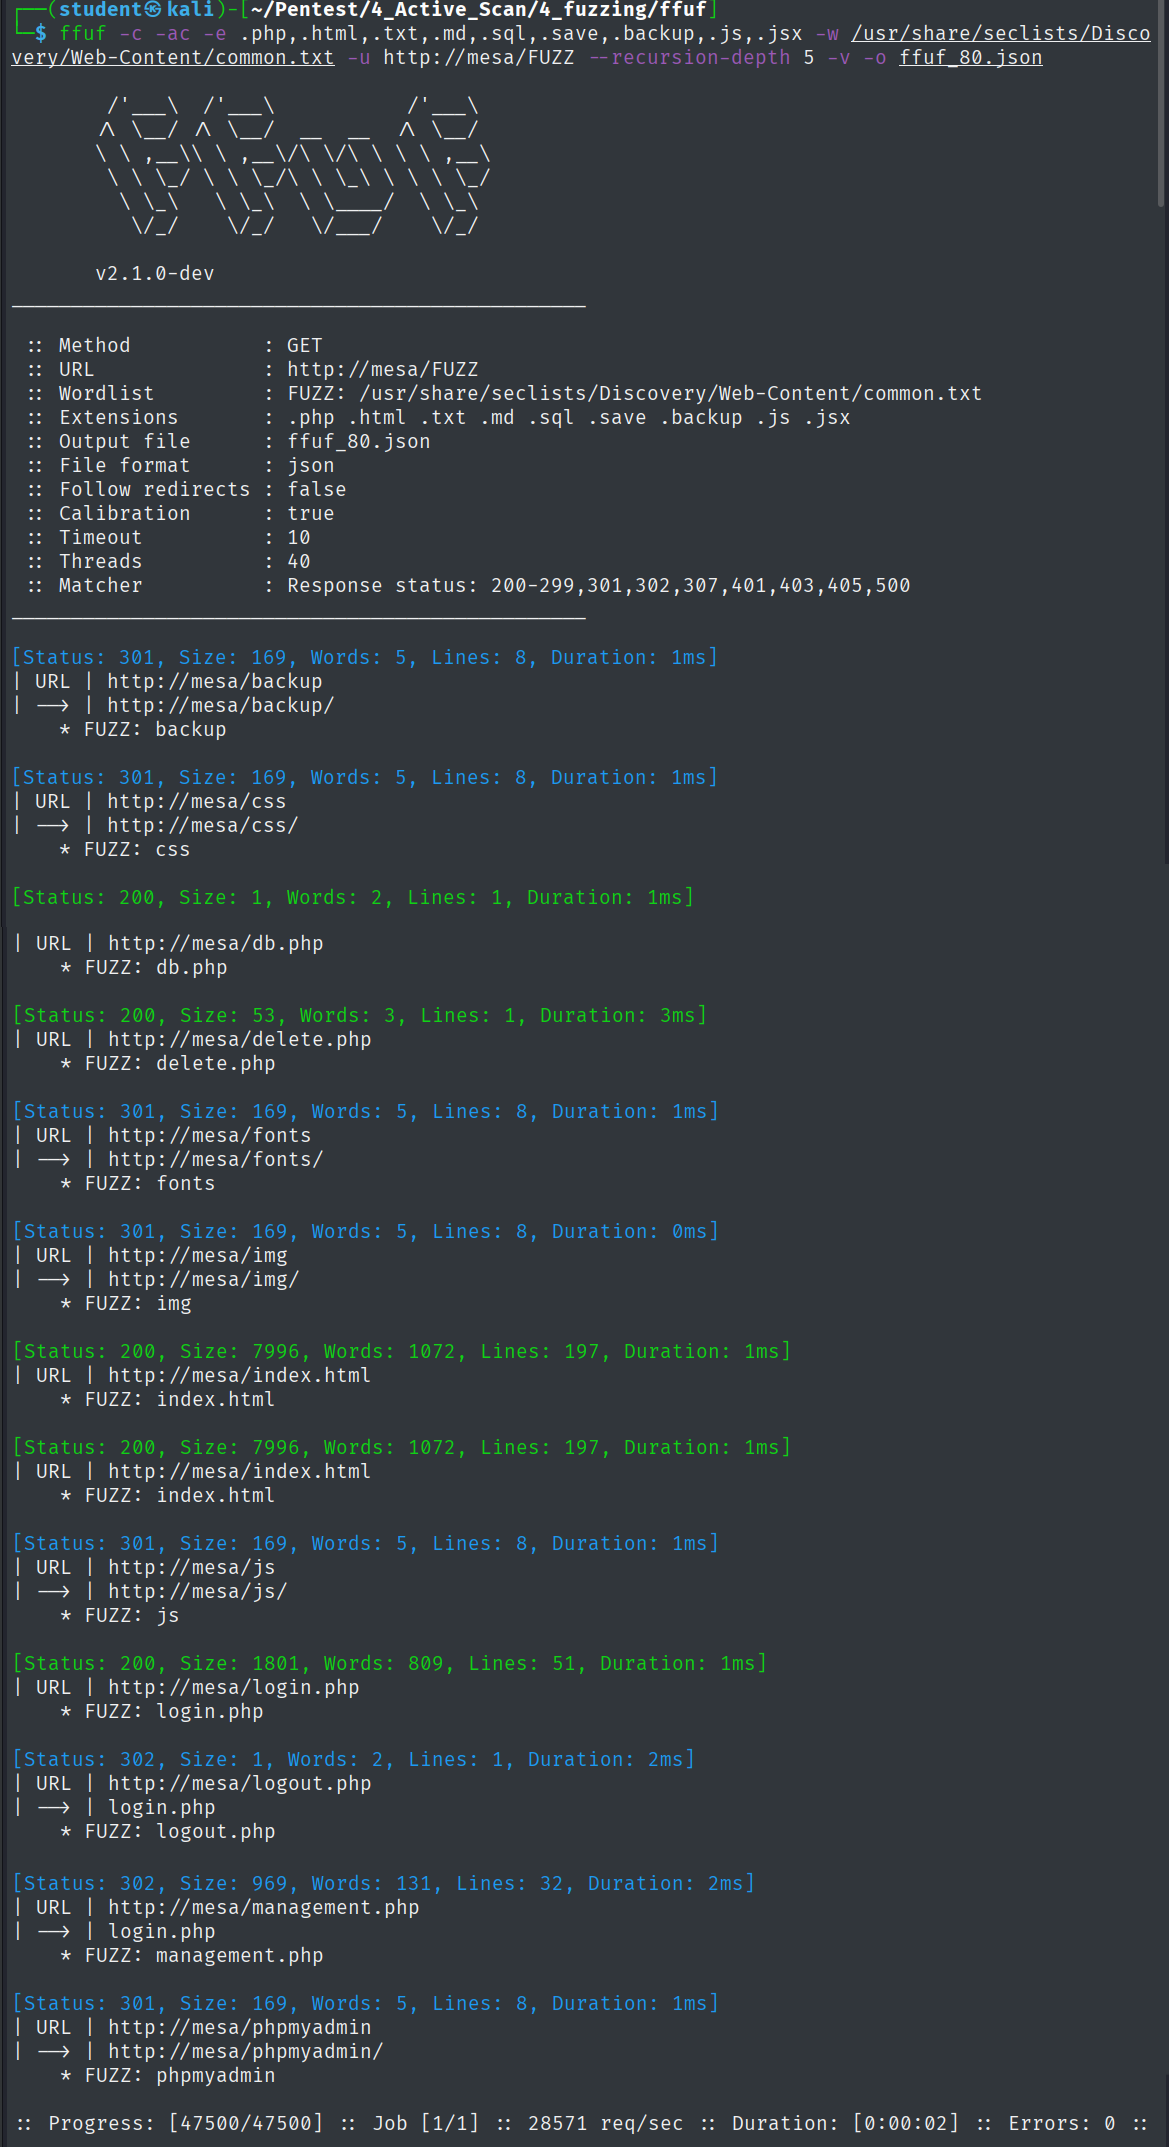
\includegraphics[width=0.75\linewidth]{pentest/1_active_scan/4_fuzzing/ffuf/ffuf}
}
\caption{Port 80 Ffuf result}
\label{ffuf_80_full}
\end{figure}

\begin{figure}[!h]
\makebox[1.01\linewidth][c]{%
	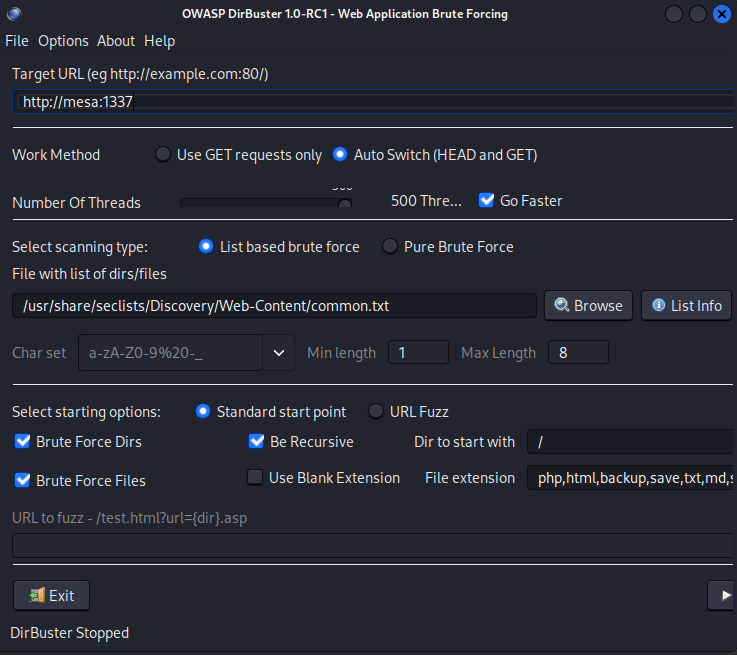
\includegraphics[width=\linewidth]{pentest/1_active_scan/4_fuzzing/dirbuster/setup/1337-setup}
}
\caption{Port 1337 scan - Dirbuster setup}
\label{dirbuster_1337_setup}
\end{figure}

\begin{figure}[!h]
\makebox[1.01\linewidth][c]{%
	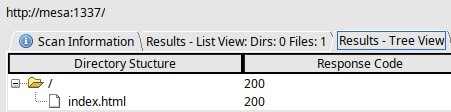
\includegraphics[width=\linewidth]{pentest/1_active_scan/4_fuzzing/dirbuster/1337-result}
}
\caption{Port 1337 scan - Dirbuster result}
\label{dirbuster_1337_result}
\end{figure}

\newpage

\begin{figure}[!htb]
	\centering
	\makebox[\linewidth][c]{%
		
\includegraphics[width=0.82\linewidth, height=21.4cm]{pentest/1_active_scan/5_technologies/80}
	}
	\caption{Whatweb results for port 80}
	\label{whatweb_80}
\end{figure}

\begin{figure}[!htb]
	\centering
	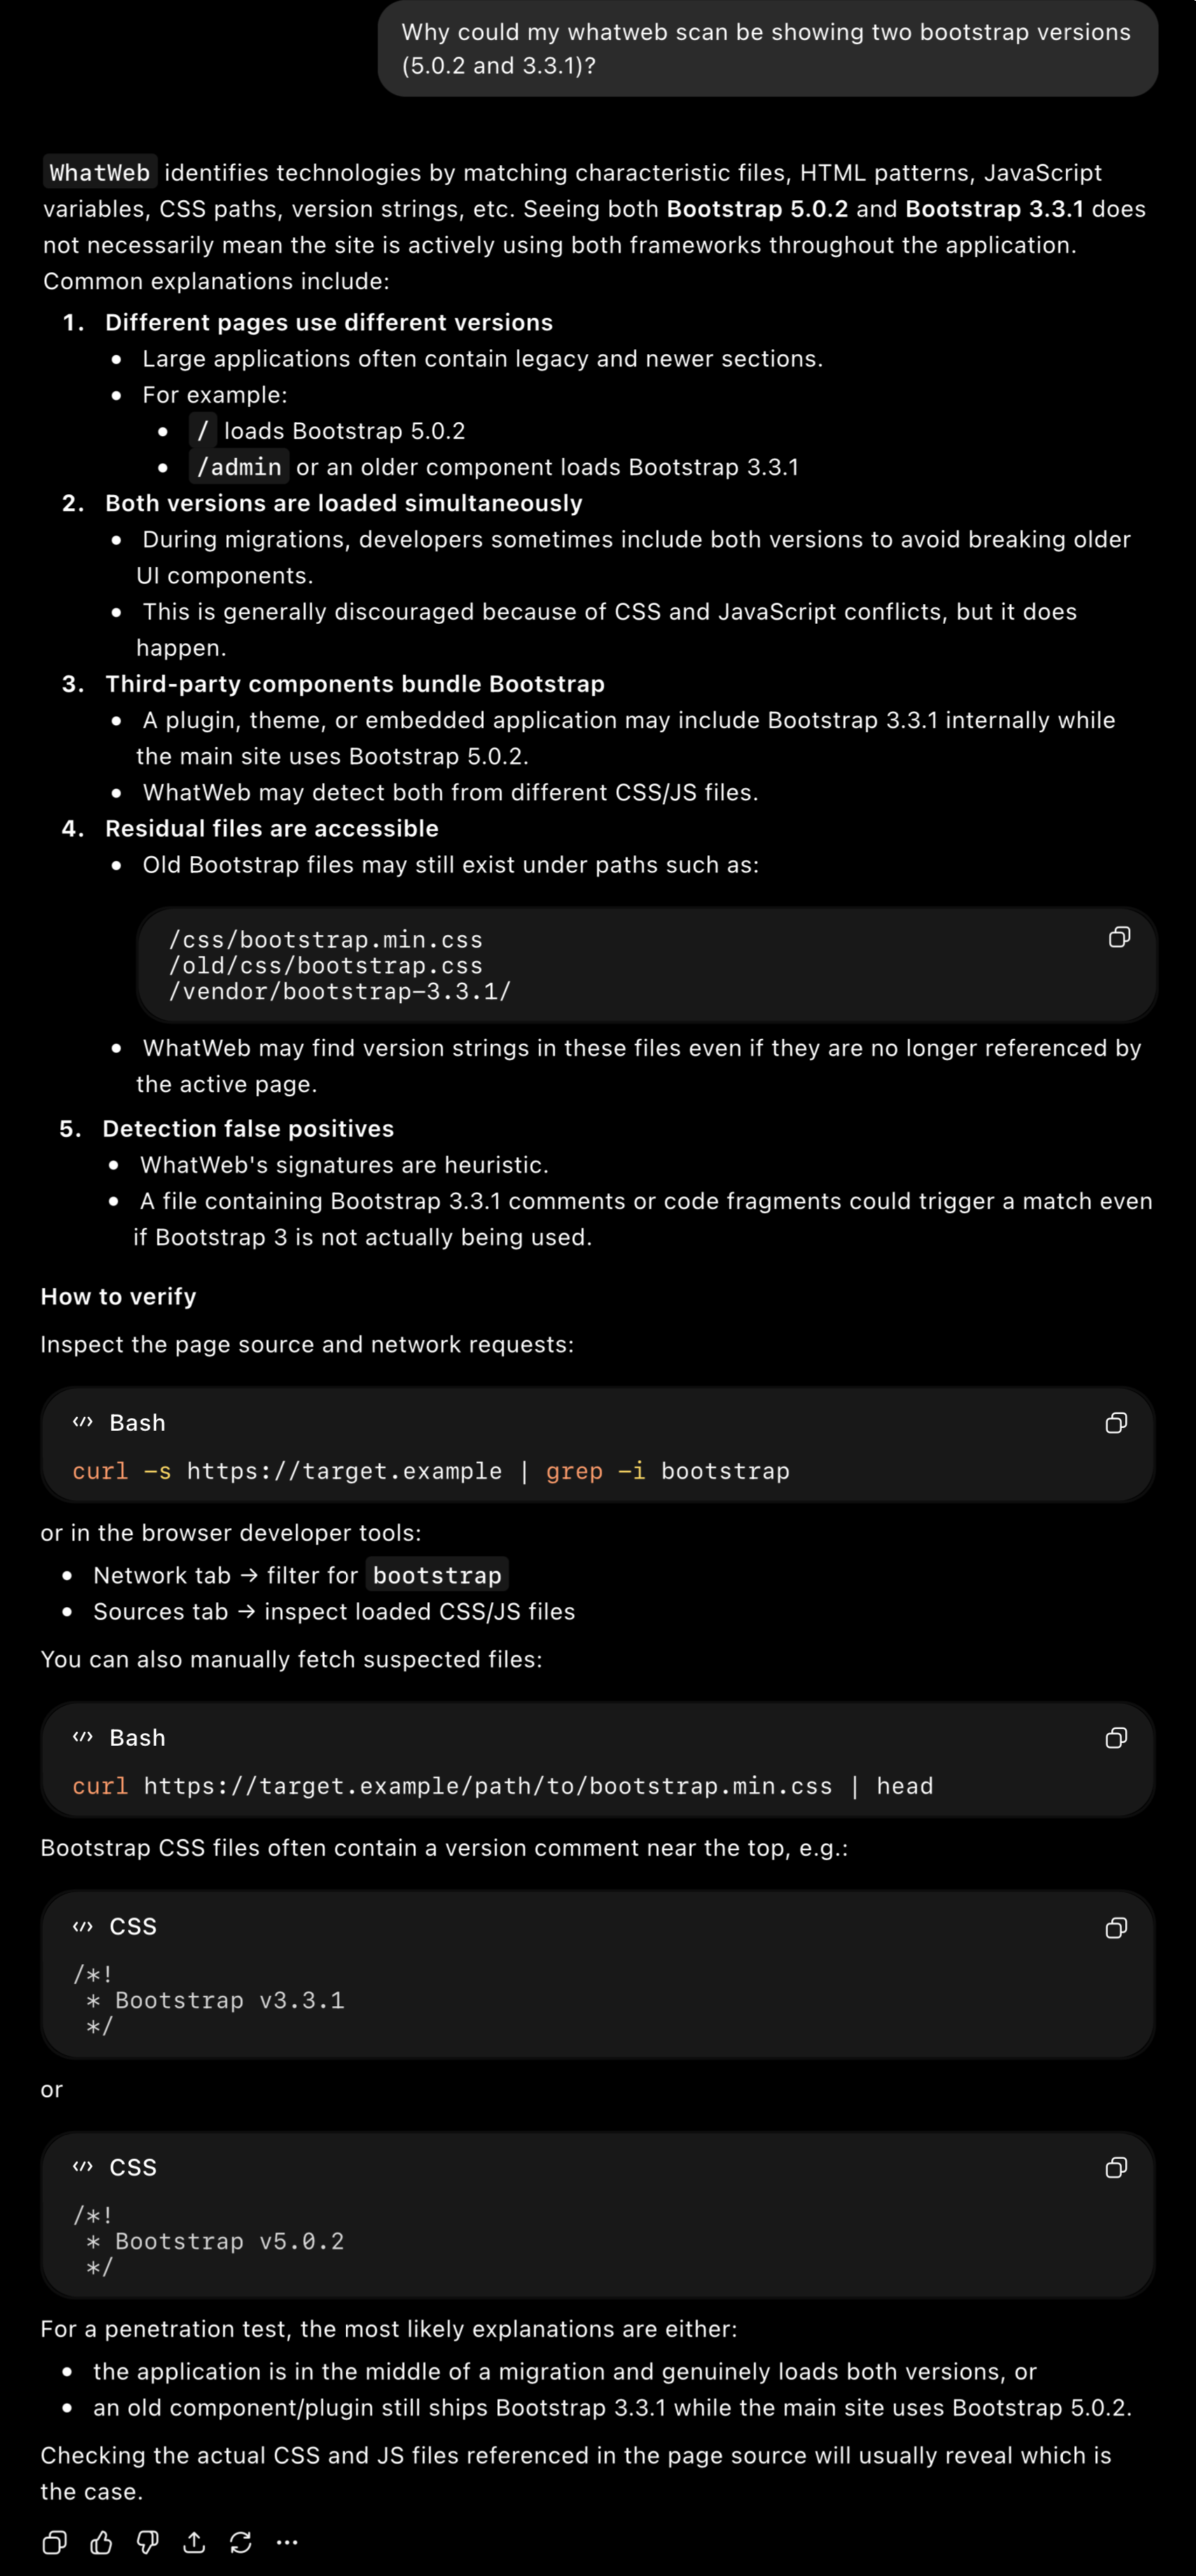
\includegraphics[width=0.62\linewidth]{pentest/1_active_scan/5_technologies/port_80/bootstrap/chatgpt}
	\caption{Whatweb - Reasons for multiple Bootstrap versions on port 80 ChatGPT log}
	\vspace{-2mm}
	\caption*{Source: \url{https://chatgpt.com}}
	\label{multiple_versions_log}
\end{figure}

\begin{landscape}

\begin{figure}[!htb]
\makebox[\linewidth][c]{%
	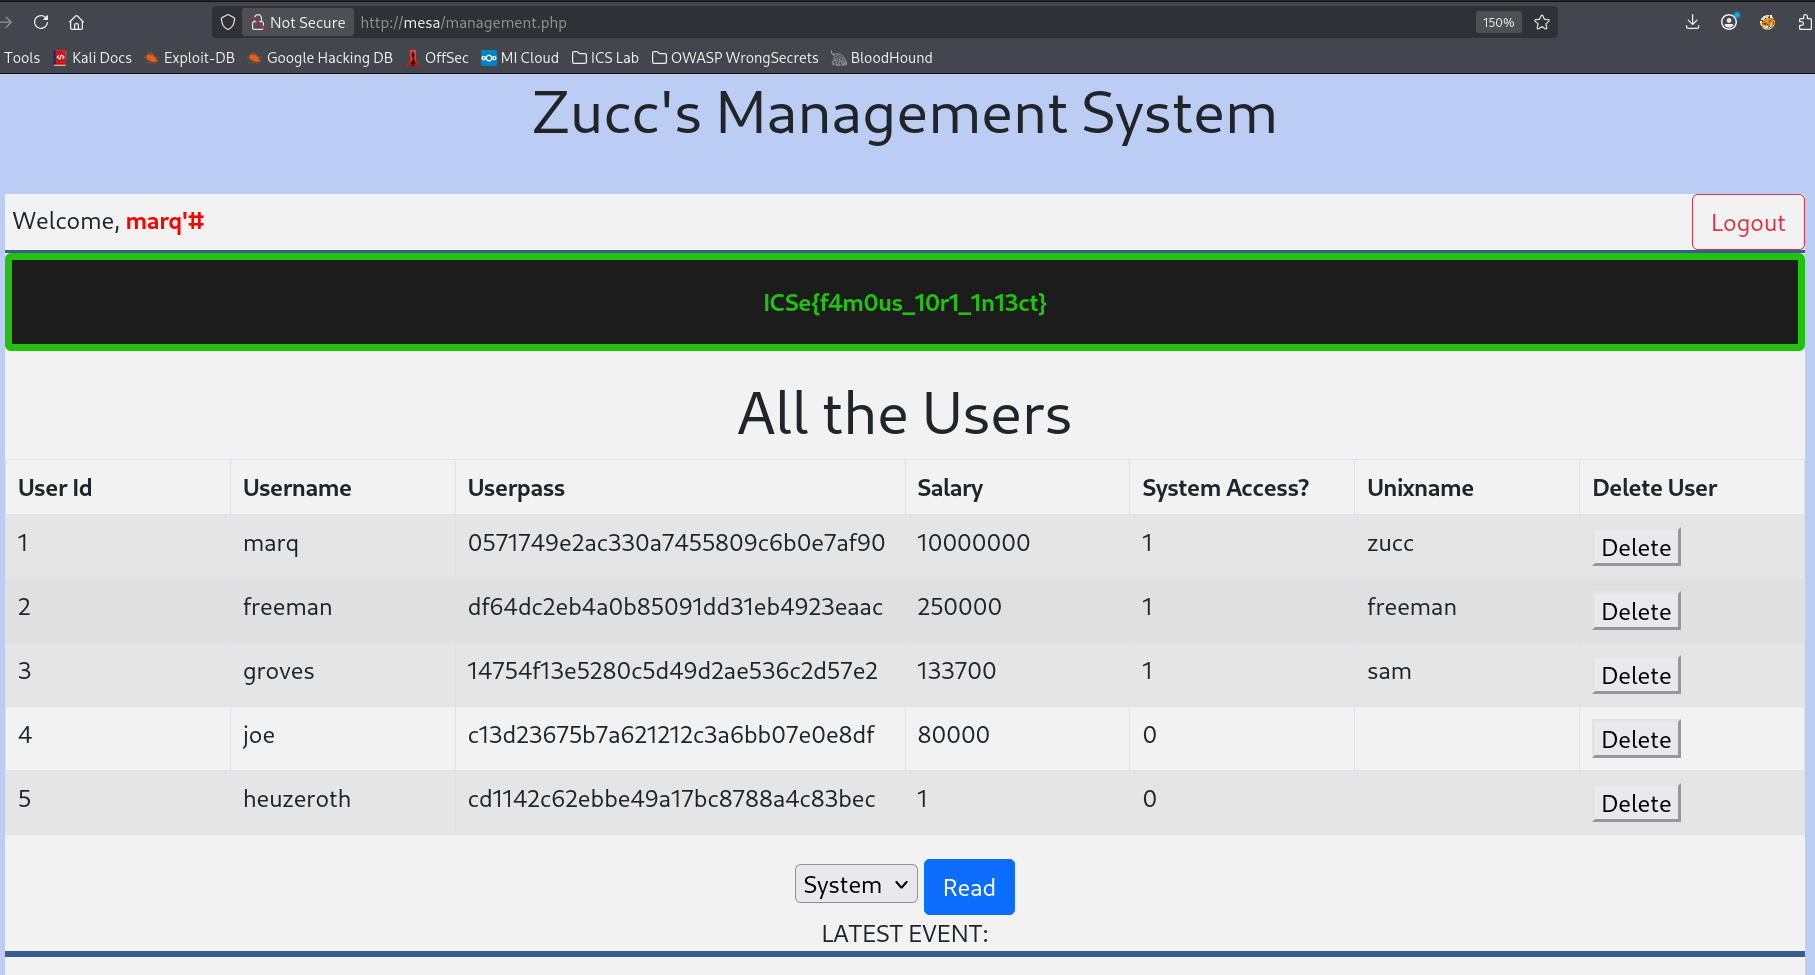
\includegraphics[width=1.15\linewidth]{pentest/2_login/sql_injection/full_inject1}
}
	\caption{Successful SQL injection attempt 1}
	\label{full_inject1}
\end{figure}

\begin{figure}[!htb]
\makebox[\linewidth][c]{%
	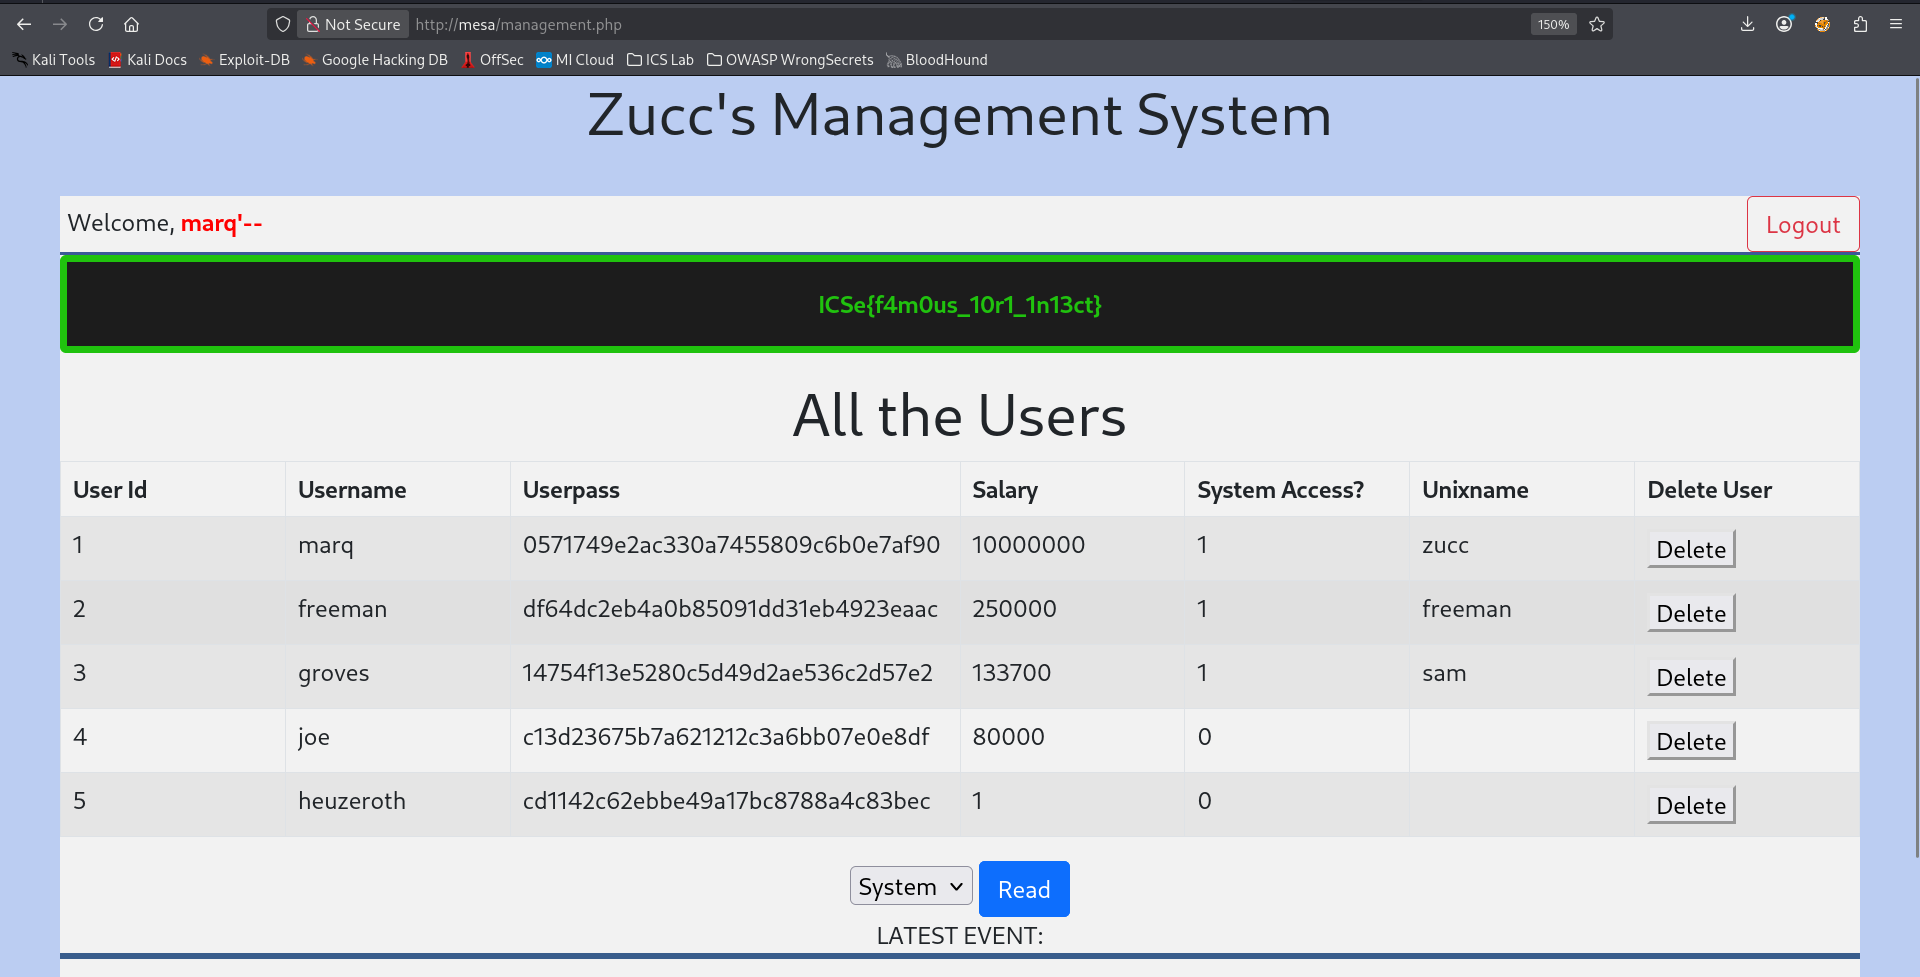
\includegraphics[width=1.15\linewidth]{pentest/2_login/sql_injection/full_inject2}
}
	\caption{Successful SQL injection attempt 2}
	\label{full_inject2}
\end{figure}

\begin{figure}[!htb]
\makebox[\linewidth][c]{%
	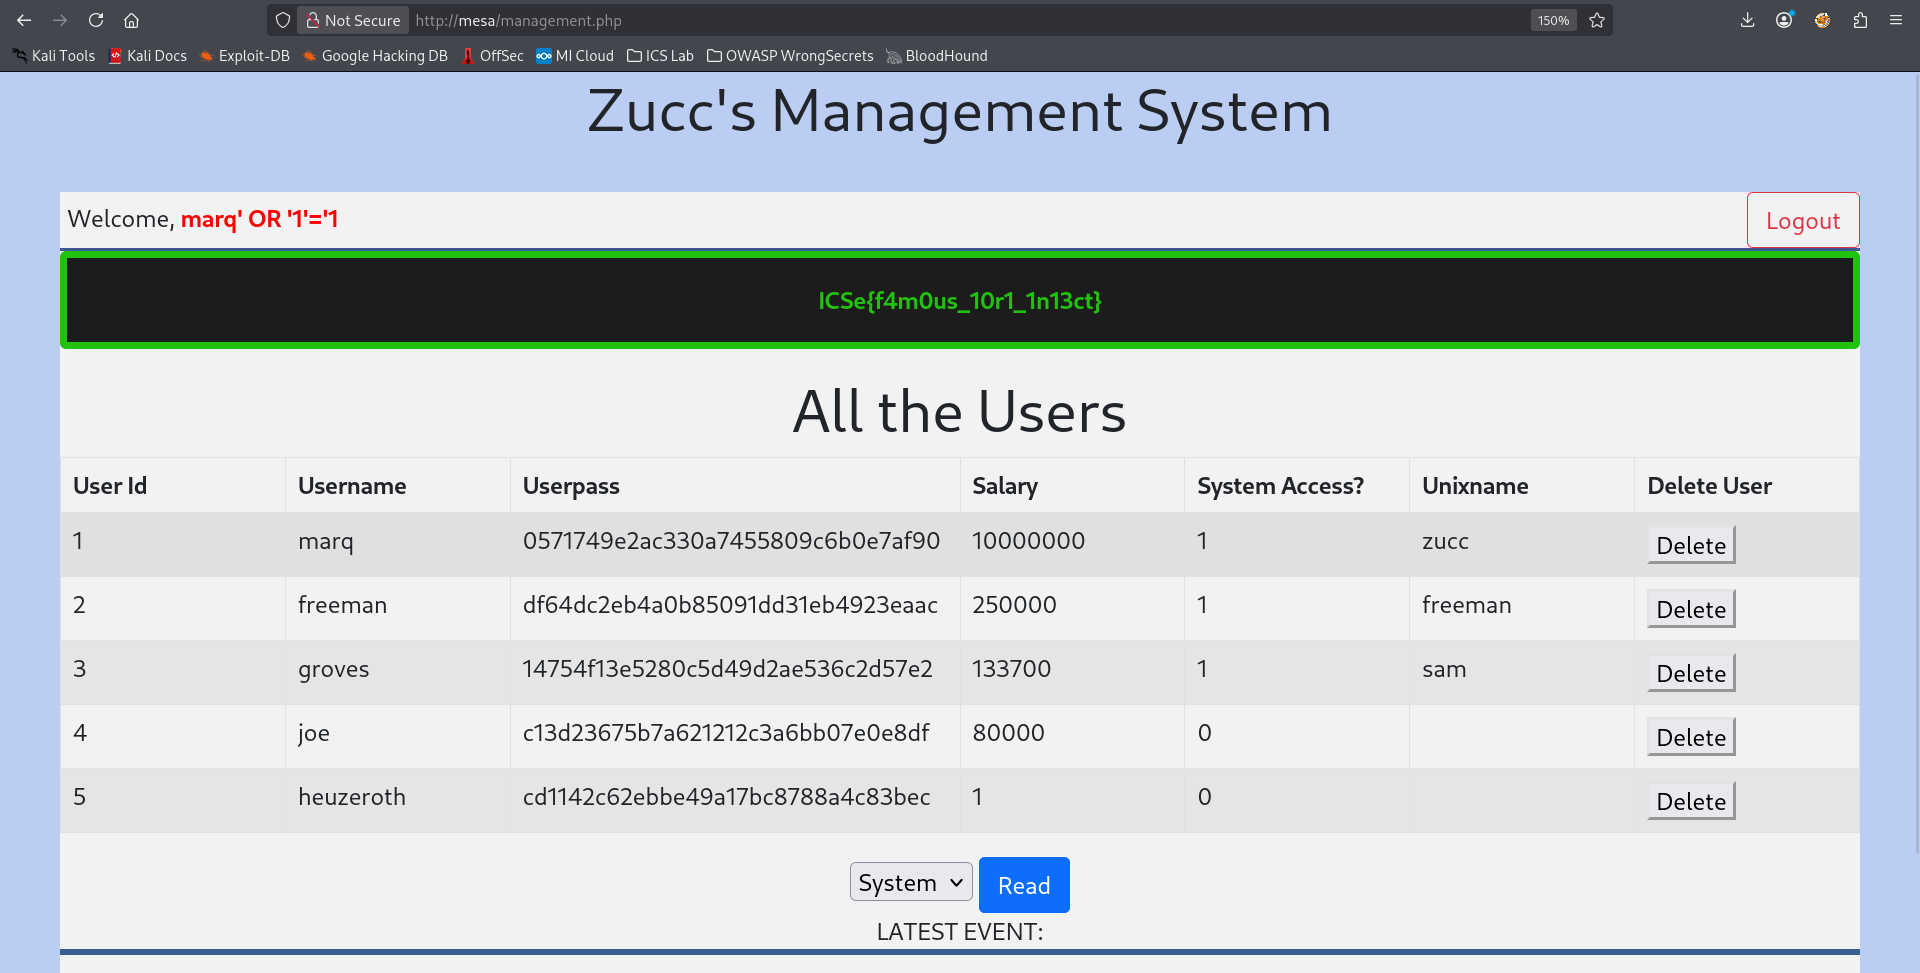
\includegraphics[width=1.15\linewidth]{pentest/2_login/sql_injection/full_inject3}
}
	\caption{Successful SQL injection attempt 3}
	\label{full_inject3}
\end{figure}

\end{landscape}

\begin{figure}[!htb]
\makebox[\linewidth][c]{%
	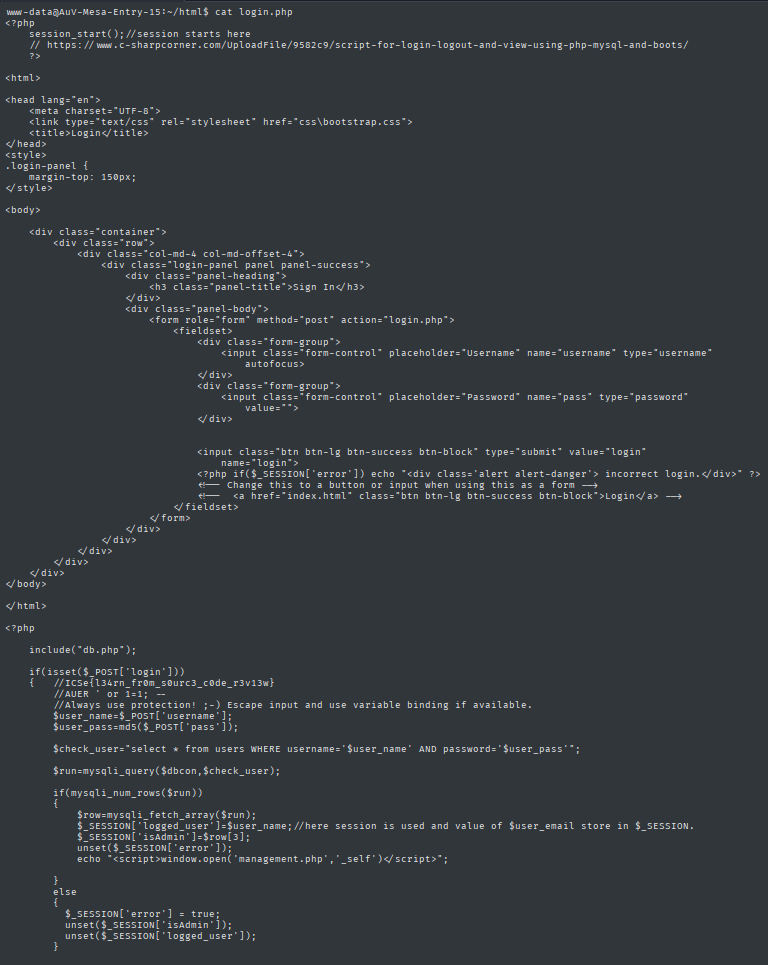
\includegraphics[width=1.1\linewidth]{pentest/4_source_code/2_login.php}
}
	\caption{login.php read via reverse shell}
	\label{login_php_full}
\end{figure}

\begin{figure}[!htb]
\makebox[\linewidth][c]{%
	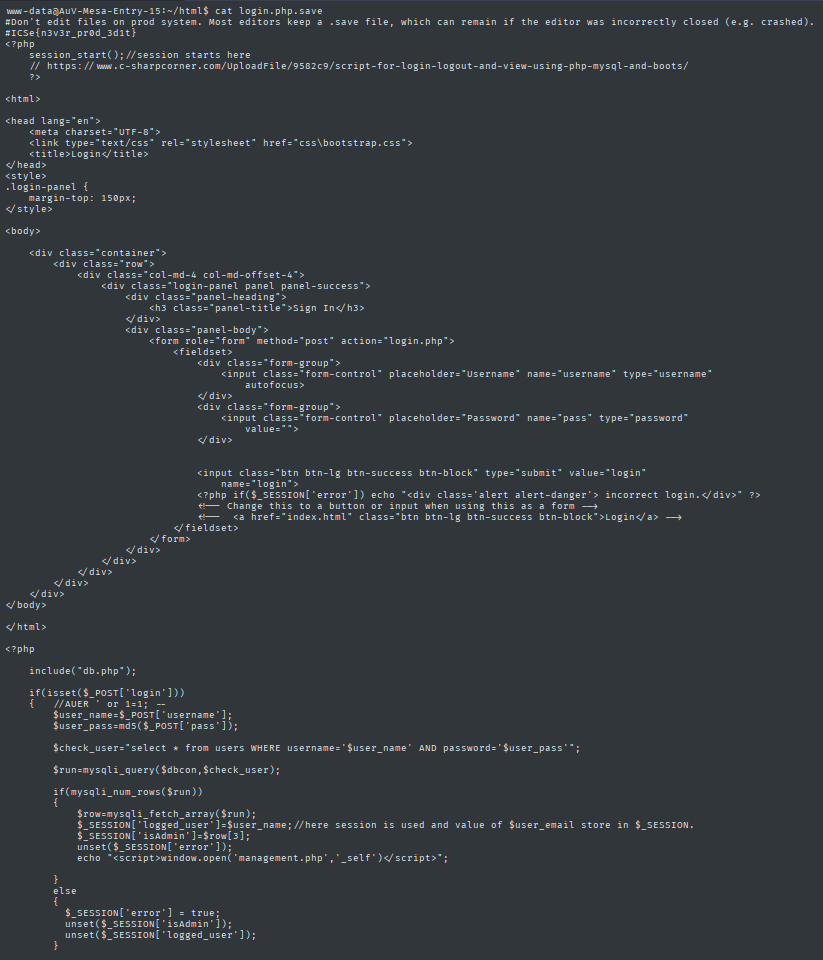
\includegraphics[width=1.18\linewidth]{pentest/4_source_code/1_login_save}
}
	\caption{login.php.save read via reverse shell}
	\label{login_save_full}
\end{figure}

\begin{figure}[!htb]
\makebox[\linewidth][c]{%
	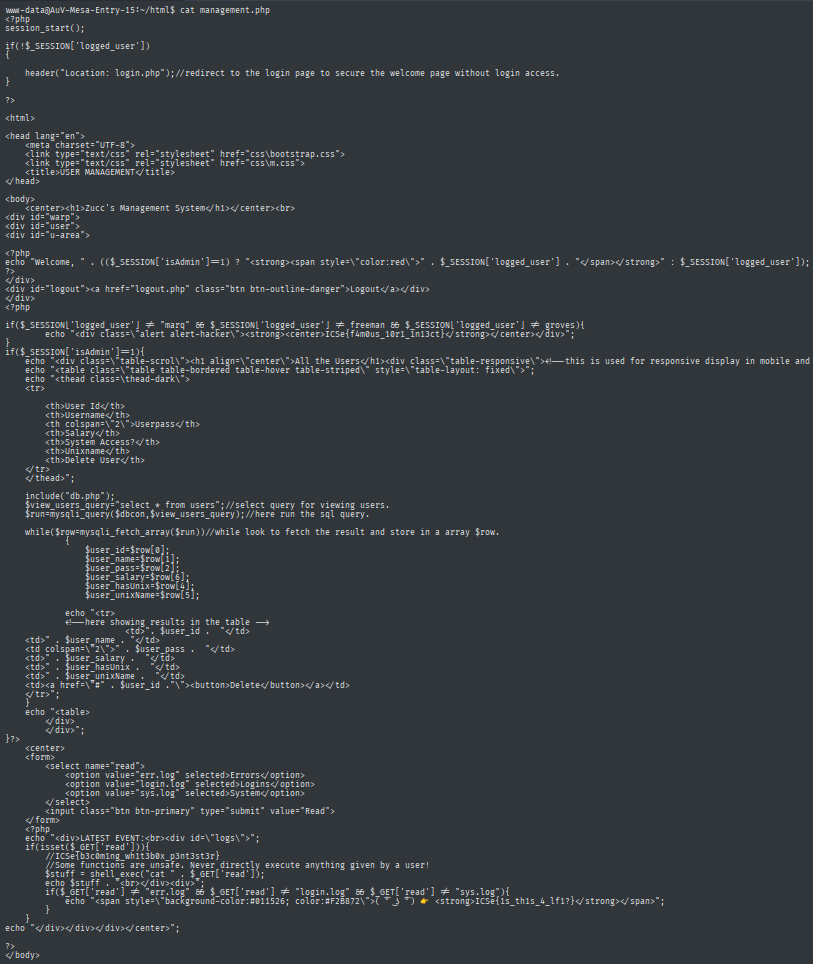
\includegraphics[width=1.18\linewidth]{pentest/4_source_code/3_management.php}
}
	\caption{management.php read via reverse shell}
	\label{management_full}
\end{figure}

\clearpage
\newpage

\subsection{Digital Forensics}  \label{Appendix-3}

\resumetoc
\end{document}